\chapter{Linked Data}
\label{ch5}
\usepackage{arabtex}
\usepackage{utf8}
\usepackage{CJKutf8}
\section{Weaving a Web of Data}



The architects  of the World Wide Web made some very specific choices in its design 
to allow it to grow to global scale.   The  Web relies on open standards to specify the components of its
architecture, allowing them to span different software and hardware, making it both implementation-independent and domain-independent. To
support a Web of data, we want to take advantage of this infrastructure as much as possible. 
By
reusing  the World Wide Web architecture, the Web of data
becomes a backward-compatible extension and evolution of the hypertext
Web and remains compatible and combinable with all the other facets of
it. The Web of data applies the Web architecture to structured data
sharing on a World Wide scale. Meanwhile, it retains its architectural
support for decentralization, extensibility and openness.


What changes do we have to make to the hypertext Web to allow the Web of data
to be able to describe  resources and publish data? As
shown in Figure~\ref{fig:ch5.1}, this requires two steps:  expanding the set of exchange formats from     HTML (and other document formats) to include  RDF and its serializations (Section~\ref{serialization}) for exchanging data, and generalizing 
URLs (Uniform Resource Locators) to URIs (Uniform Resource Identifiers) 
or IRIs (Internationalized resource identifiers), to identify and then describe virtually anything. ,

\begin{figure}
    \centering
    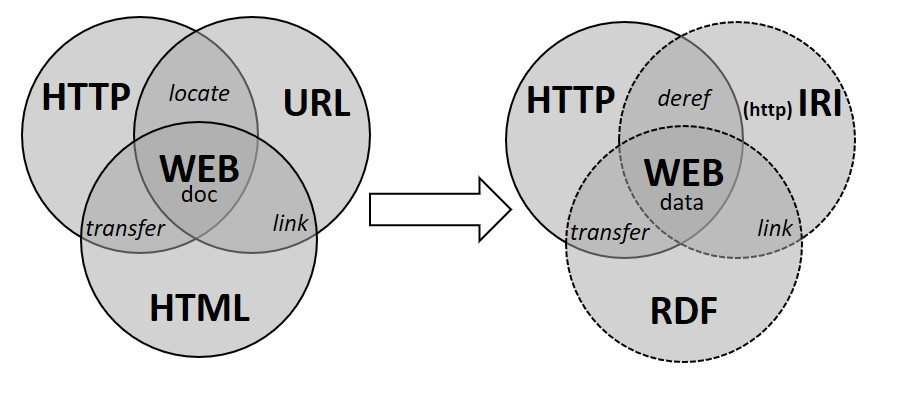
\includegraphics[width=5.0in]{media/ch5/figure-05-01.jpg}
    \caption{Relying on the Web architecture to publish linked data}
    \label{fig:ch5.1}
\end{figure}


Publishing data on the Web is not only about dumping data somewhere on
the Web, it also means linking data so that it can be found, browsed,
crawled, integrated, etc. So in a Web of data, the core idea is the one
of \emph{linked data}, i.e. datasets (and data elements in them)  linked across the
World Wide Web in the same way Web pages, Web sites and anchored texts
are linked across the World on the Web. Instead of just
using HTML to write Web pages that inlcude links to other pages, the Web of
data uses RDF to write data descriptions that include links to other data
descriptions.

Tim Berners-Lee introduced best practices for linked data in his
personal notes on Linked Data Design Issues in 2006\footnote{Linked
  Data, Tim Berners-Lee, 2006-07-27,
  https://www.w3.org/DesignIssues/LinkedData.html}, stating the
architectural principles and explaining the thinking behind the linked data
specifications.   In this chapter, we will explain in detail his three rules 
for data publication that will allow us to weave a web of data:



\begin{enumerate}
\def\labelenumi{\arabic{enumi}.}
\item
\label{ruleURI}
  Use HTTP URIs to name everything: Just as URLs were introduced to
  address and locate resources on the Web, the Web of data uses URIs to
  name the things it describes. But by using HTTP URIs we can also
  provide a default mechanism to obtain descriptions: HTTP URIs are
  names (URIs) supporting lookup (HTTP access). This allow us to
  look up the name of the things they identify.
\item
\label{ruleFYN}
  When an agent accesses an HTTP URI, the server must provide descriptive
  information about the resource identified by that URI using the Web
  standard languages, in particular RDF and its syntaxes.
\item
\label{ruleLink}
  In the descriptive data it provides, a server must include links to
  HTTP URIs of other things so that Web clients can discover more things
  by looking up these new HTTP URIs recursively at will.
\end{enumerate}

These simple rules are a natural extension of how thy hypertext Web works. When we put a hypertext page 
on the web, use an HTTP URI (URL) to reference it.  When an agent accesses that HTTP URI, the server provides 
the page itself.  A hypertext page refers to other pages by including links to their HTTP URIs. 
For the hypertext web, this makes the pages interconnected; from any page an 
information consumer can access others.

By applying these  rules to the Web of data, we make it interconnected in the same way.  
when we use an HTTP URI   for our data elements (rule \ref{ruleURI}), 
we make it possible for anyone on the web to reference them. Once someone
(re-)uses one of our HTTP URIs , their dataset and ours
are interconnected.  When we include links in our data to 
other data sets (rule \ref{ruleLink}) and  describe our own 
datasets (rule \ref{ruleFYN}), we make 
the interconnected data \emph{discoverable}, that is, 
someone coming to one data set can discover another
without having to search for it. 


\hypertarget{calling-a-cat-an-httpcat}{%
\subsection{Calling a cat an
http://cat}\label{calling-a-cat-an-httpcat}}

When we expand the hypertext web into a full Web of data, instead of just using URLs to 
identify what exists on the web (\url{http://my-site.fr}), we also start using
URIs to identify, on the web, what exists in general
(e.g., \url{http://animals.org/cat\#mytsie}, for Fabien's cat, Mytsie).  As we include IRIs in the Web of data, we identify,
on the web, what exists, in any language
(e.g., http://\<الحيوانات.tn/ >.tn/\begin{CJK*}{UTF8}{gbsn}猫
\end{CJK*}\#mytsie).



The distinction between identifying what is on the Web vs. identifying
on the Web anything that exists, is much more than a play on words.
Instead of just using the Web to exchange data about its own content, we
can use it to exchange data about anything around us: a page, a person,
a car, a cat, an idea, a country, a product, a service, a policy, a
relation, etc.

In the acronyms URL, URI and IRI the `R' stands for ``Resource''. In the
Web architecture a resource is anything that can be identified. And in
practice, URIs are now used to name a lot of very different things. Here
are some examples:

\begin{itemize}
\item
  URI for Paris in DBpedia: \url{http://dbpedia.org/resource/Paris}
\item
  URI for the protein MUC18 in UniProt:
  \url{http://www.uniprot.org/uniprot/P43121}
\item
  URI for the name of Victor Hugo in the Library of Congress:
  \url{http://id.loc.gov/authorities/names/n79091479}
\item
  URI for Xavier Dolan in Wikidata:
  \url{http://www.wikidata.org/entity/Q551861}
\item
  URI for Fabien Gandon at Inria:
  \url{http://ns.inria.fr/fabien.gandon\#me}
\item
  URI for the "31st of December 2016 at 23:00 in New York":
  \url{http://www.timeanddate.com/worldclock/meetingdetails.html?year=2017\&month=1\&day=1\&hour=4\&min=0\&sec=0\&p1=179}
\end{itemize}

The reliance on URIs is key to distributed data, to the Web\-based
architecture and to the integration of datasets coming from different
sources and produced by different means.

URIs  allow us to make  vocabulary and  resource
identification unambiguous by providing a global identification
mechanism for the terms and subjects of our descriptions. URIs also have a 
\emph{deferencing} mechanism, that is, a method that uses the URI to find a location 
on the web from which further information can be loaded. 
Applications use this universal
identification mechanism to ensure they are processing the right data,
in the right way and they use the dereferencing mechanism to obtain more
data on demand.

When URIs are used and reused across RDF graphs and datasets, they
provide junction points that allow us to merge the datasets regardless
of their provenance, potentially forming a  giant global graph. This
extensible nature of RDF graphs provides a way to weave a World-Wide Web
of data.

\subsection{Things, Representations and Identifiers}
\label{usehttp}
When we use URLs for Web resources alongside URIs for things, we can
leave our datasets open to some confusion. For example, if we use the
same URI for a cat and for a document about that cat, as soon as we
start attaching descriptions to that URI we need to know precisely what
we are talking about. For instance, if we attach a property to that URI
to provide a ``size'' it is important to know if it refers to the size of the
cat or the size of the document about the cat. For this reason, the best
practice is to use different URIs to identify different resources, and
to realize that a cat and a document about that cat (or a picture of
that cat) are not the same thing. Then, relying on the standard
mechanisms of the Web architecture we can learn more about these
different URIs and their link and for instance, as we will see in the
next section, how to obtain the URL of a document about a cat from the
URI identifying that cat (see Figure~\ref{fig:ch5.cats})

\begin{figure}
    \centering
    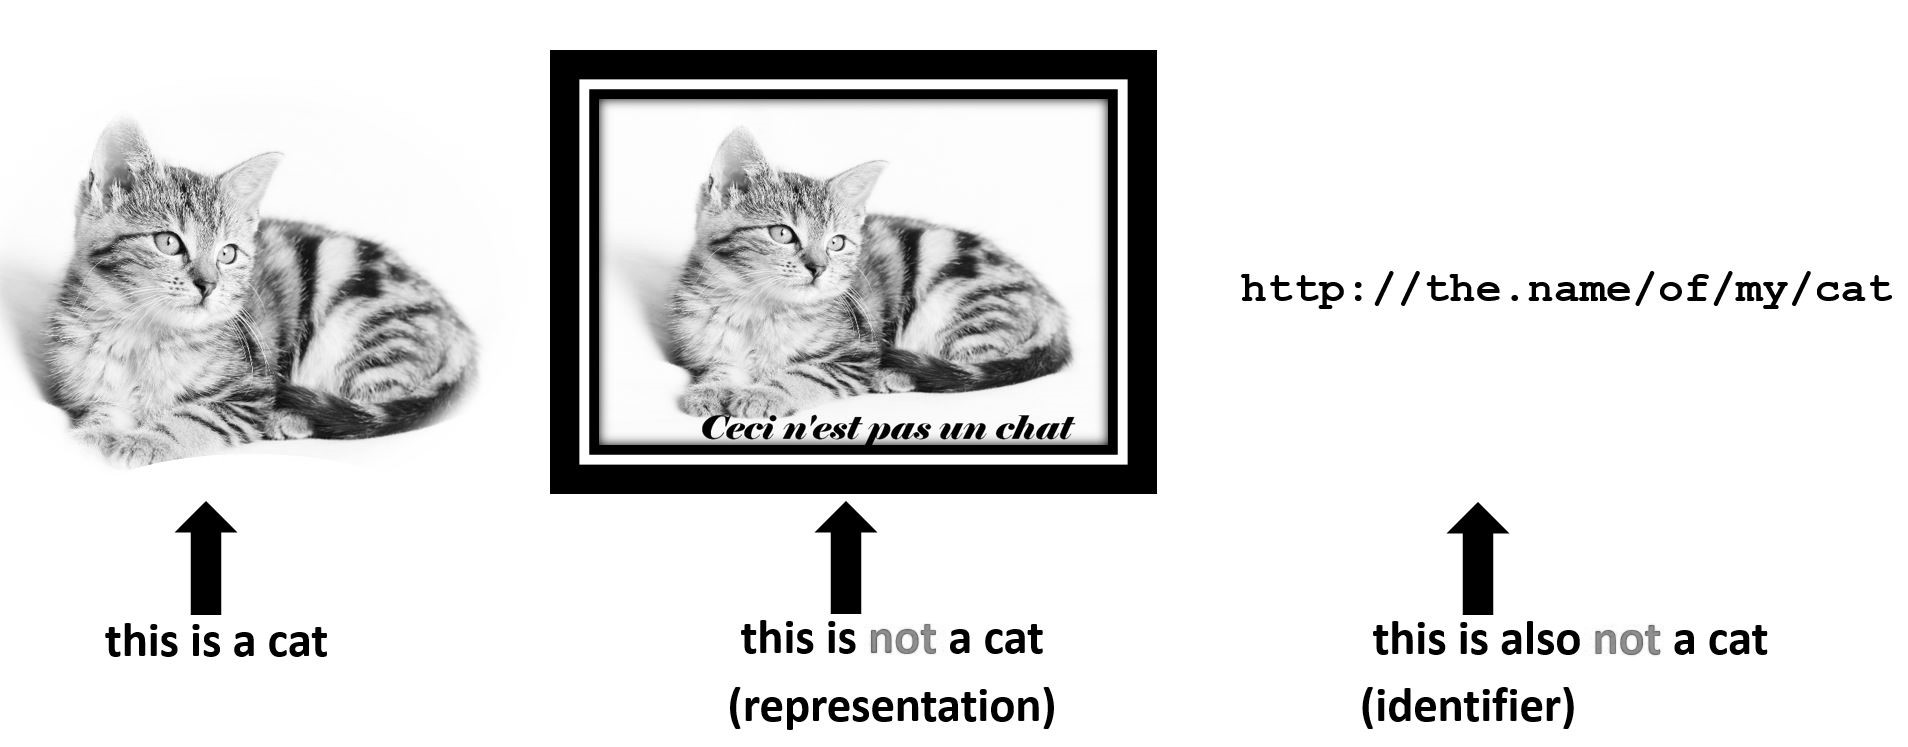
\includegraphics[width=5in]{media/ch5/WebAndCats.jpg}
    \caption{The difference between a cat, a picture of a cat, and an identifier for that cat.  Good linked data practice suggests using an identifer that can be used to look up the picture. }
    % free for commercial use, see https://pixabay.com/en/cat-pet-striped-kitten-young-1192026/
    \label{fig:ch5.cats}
\end{figure}

\hypertarget{dereferencing-http-uri}{%
\subsection{Dereferencing HTTP URI }\label{dereferencing-http-uri}}

An HTTP URI is a URI created to name anything we want to talk about 
that  uses  HTTP   as its dereferencing mechanism. When a person or a
software agent (e.g. a Web crawler) comes across that URI, they can easily learn more
about the resource it represents,  by simply making an HTTP call
to the address it provides.   Dereferencing of HTTP URIs is a cornerstone of the hypertext web, and has
functioned well since the beginning of the Web. HTTP URIs come with an
obvious way to get a description about the resource they identify: the
HTTP protocol that can be used to looked them up. Other URI schemes
(e.g. URN, DOI, etc.) require additional services or practices to be
dereferenced.  

We don't use the term URL (Uniform Resource \textbf{Locator}) for these identifiers, to emphasize the 
point that the thing  being
represented may not itself be on the Web at this address, or even at on the Web at all. For example, I
may want to specify an HTTP URI for my cat Mytsie. No matter how hard I
try, Mytsie herself will never be located on the Web, so I cannot give
her a URL \emph{per se}. But this adorable cat can be identified on the
Web by an HTTP URI and if you ever go to that address you will be
provided with a description (maybe even a photo or two) on the Web about the resource represented by
that URI, i.e. my cat Mytsie.

This approach to linked data, in which we use an HTTP URI as an identifier, and 
rely on HTTP-based dereferencing of that URI to provide more information about the resource, 
is summarized in a web design pattern called \emph{Follow Your Nose} \footnote{Linked Data Patterns, by Leigh Dodds and Ian Davis,
http://patterns.dataincubator.org/book/follow-your-nose.html}.
According to the  Follow Your Nose pattern,  it is the responsibility of the data publisher
to make sure that the HTTP URIs indeed resolve to web resources that provide
appropriate information. Just as Ariadne provided Theseus a thread to let him
find his way back out of the labyrinth, the web publisher provides HTTP URIs
that allow data consumers to find their way back to the data source, to
learn more about it.  It is up to the data consumer and the details of their application (including issues around performance, trust, scalability,
quality, etc.)
whether they want to follow these links at any particular time. 


Since HTTP URIs rely on the domain names to create the first part of the
URI scheme, they support the decentralized creation of globally unique
identifiers. Any owner of a web domain can create and control the access to
any HTTP URIs in that domain. In choosing and using HTTP URIs, there are
three important standard mechanisms of the Web and Internet to be aware
of: the Domain Name Service (DNS) and its implication on the choice of
domain part of the URIs; content negotiation in HTTP, which allows a
server to serve different contents for the same HTTP URI to different
clients; and HTTP redirection, which allows a server to redirect a call
to another address. These three mechanisms and their impacts are
illustrated in figure~\ref{fig:ch5.2} and detailed in the next sections.



\begin{figure}
    \centering
        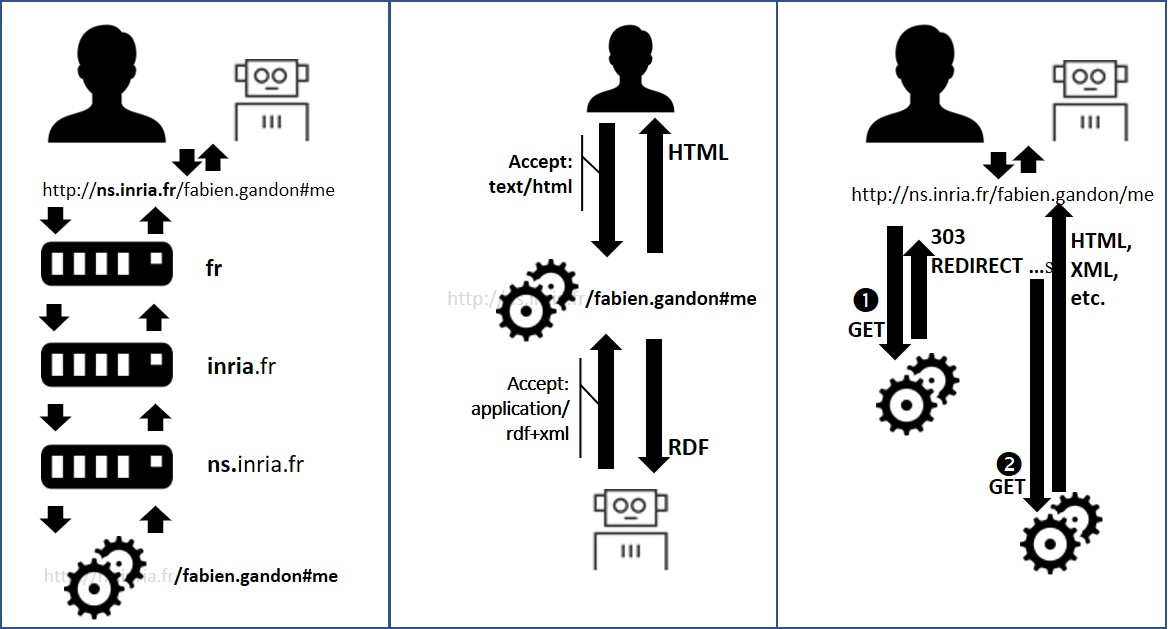
\includegraphics[width=5.0in]{media/ch5/figure-05-02.jpg}
    \caption{Three standard mechanisms used in Web Data publishing and
accessing}
    \label{fig:ch5.2}
\end{figure}


\hypertarget{minting-http-uris}{%
\subsection{Minting HTTP URIs}\label{minting-http-uris}}

How do we choose the URIs we are going to use to talk about the things
we want to describe? What should be their structure or naming schema?
Are there criteria and pitfalls in choosing a method to create URIs for
our collections and applications? These questions are legitimate since
as soon as we start publishing URIs they are reused and referenced and
therefore introduce dependencies and create legacy systems.

The generic form of a URI is describe in their standard
document\footnote{URIs are standardized in RFCs from IETF : RFC 3986
  https://tools.ietf.org/html/rfc3986} like this where values between
square brackets are optional parts one can use in minting a URI (eg.
Indicating a port on a server).

\begin{lstlisting}
scheme:[//[user:password@]host[:port]][/]path[?query][#fragment]
\end{lstlisting}

For instance, a valid URI according to this pattern is for instance:

\begin{lstlisting}
urn:animals.org\#mycat
\end{lstlisting}

As we saw in Section~\ref{usehttp}, using HTTP URIs is preferring for the web 
of data, in contrast to other protocols.  An HTTP URI has the form: 



\begin{lstlisting}
http://host[:port]][/]path[?query][#fragment]
\end{lstlisting}


For instance, the following are valid HTTP URIs:

\begin{lstlisting}
http://animals.org#mycat
http://animals.org/cats/mine
http://animals.org/cats/?owner=fabien
...
\end{lstlisting}


Within a single domain (which corresponds to the \emph{host} in the HTTP protocol, 
the \emph{path} part of the HTTP URI can be arbitrarily long, therefore. 
no practical limit on the number of possible URI patterns we have at our disposal to name the things we
want to describe on the Web. 

\subsetcion{How to build a URI}

Since we are using HTTP URIs for all our data elements, we need to have some 
method for how we will generate enough distinct URIs for everything we want to describe in our data. 
The problem of coming up with appropriate identifiers in a large data set is not 
specific to the Semantic Web, and there is no perfect answer. In the context of HTTP URIs for the Semantic Web,
Pros
and Cons have been discussed in several places\footnote{Cool URIS:
  \url{http://www.w3.org/TR/cooluris/} and Issue 57:
  \url{http://www.w3.org/2001/tag/awwsw/issue57/latest/}}.  We will
summarize here some of the things to consider when minting your HTTP
URIs. 


Inspired by the title of an article by Tim Berners-Lee, \emph{Cool URIs don't change}, \footnote{Cool URIs don't change, Tim Berners-Lee, 1998.  http://www.w3.org/Provider/Style/URI.}, a popular proposal for 
minting URIs for the semantic Web is called \emph{Cool URIs}

As suggested by the eponymous article, a key aspect of cool URIs is that they don't change: you want to ensure
that your URIs will be as stable as possible by choosing a stable URI pattern. 
Why is it important to have stable URIs?  
While the ``404 page not found'' error is disappointing on the hypertext web, it can be catastrophic in the Web of Data, wherethe URIs are the
linkage points between data sets.  A broken link can mean loss of access to an entire data set.

The Cool URI proposal has some advice for how to make URIs stable:

\begin{itemize}
    \item Desing URIs with reference to as few implementation details as possible. In particular, avoid language dependent extensions (.PHP, .json, .rdf), specific server names "desktop8.inria.fr", specific software (\ldots{}/wordpress/\ldots{}), server port number, etc.  
    \item Web servers are able to negotiate content based on information from web clients. Use this feature to avoid implementation details in URIs.
    \item Leave out version information from stable URIs.  The semantic web standards provide ways to specify the version of a data or metadata set, other than changing URIs. 
    \item in many cases, the original data source has some kind of identifier already (a primary key, or an account number, etc.).  You can make use of these to ensure that your URIs correspond to the right data elements. 
\end{itemize}



For example, imagine  we have a table of animals (e.g. a CSV file) with columns
providing information about the vaccination records for our pets, as shown in Table~\ref{tab:ch5.pets}

\begin{table}
    \centering
    \begin{tabular}{|l l l l|}
    \hline
    ID&Species&Name&Expiration Date \\
    \hline\hline
366863&dog&Fido&2020 \\
851903&dog&Bastian&2021 \\
775304&cat&Mytsie&2019 \\
898202&cat&Corvus&2021 \\
847823&cat&Fenris&2019 \\
399378&dog&Maddie&2022 \\
911236&cat&Twinkie&2016 \\
897991&dog&Champ&2019 \\
032579&dog&Zeke&2020 \\
31450&cat&Nix&2019 \\
87580&dog&Fido&2021 \\
\hline
    \end{tabular}
    \caption{Sample data about the vaccine records for our pets. }
    \label{tab:ch5.pets}
\end{table}


The data about the Pet's name and the expiration date of the vaccine cannot be counted on to be  unique
(in this short sample, we have two dogs named Fido).  One option for minting URIs for this would be to include all the data in each URI, as in Table~\ref{tab:ch5.all}.

This method is guaranteed to ensure uniqueness in the data, but makes for very long URIs, and can be misleading if any of the data changes.  Should we coin new URIs?  Or re-use the old ones, which will then reflect out-of-date data?

\begin{table}
    \centering
    \begin{tabular}{|l|}
    \hline
    URI \\
    \hline\hline
http://www.example.com/vac/366863/dog/Fido/2020 \\
http://www.example.com/vac/851903/dog/Bastian/2021 \\
http://www.example.com/vac/775304/cat/Mytsie/2019 \\
http://www.example.com/vac/898202/cat/Corvus/2021 \\
http://www.example.com/vac/847823/cat/Fenris/2019 \\
http://www.example.com/vac/399378/dog/Maddie/2022 \\
http://www.example.com/vac/911236/cat/Twinkie/2016 \\
http://www.example.com/vac/897991/dog/Champ/2019 \\
http://www.example.com/vac/032579/dog/Zeke/2020 \\
http://www.example.com/vac/31450/cat/Nix/2019 \\
http://www.example.com/vac/87580/dog/Fido/2021 \\
\hline
    \end{tabular}
    \caption{Coining URIs by repeating all the data }
    \label{tab:ch5.all}
\end{table}

Since the original data includes an \textbf{ID} field, we can rest assured that this 
will uniquely identify a vaccination, so we can use it for the URI, as in Table~\ref{ch5.id}

\begin{table}
    \centering
    \begin{tabular}{|l |}
    \hline
    URI \\
    \hline\hline
http://www.example.com/vac/366863 \\
http://www.example.com/vac/851903 \\
http://www.example.com/vac/775304 \\
http://www.example.com/vac/898202 \\
http://www.example.com/vac/847823 \\
http://www.example.com/vac/399378 \\
http://www.example.com/vac/911236 \\
http://www.example.com/vac/897991 \\
http://www.example.com/vac/032579 \\
http://www.example.com/vac/31450 \\
http://www.example.com/vac/87580 \\
\hline
    \end{tabular}
    \caption{Coining URIs using the ID field }
    \label{tab:ch5.id}
\end{table}


In order for this method to work, we have to make sure that the column we use really is a unique  identifier. 
For example, we might be tempted to use the column \texttt{name} to coin our URIs.  
This will cause two problems: 

\begin{itemize}
    \item we will end up coining 
\texttt{http://www.example.com/vac/Fido} twice, which will not correctly reflect the data. 
\item Even if there is no  name duplication in our data, one of the animals (say, Mytsie) might be adopted and given a new name (``Missy'').  If this happens, do we have to create a new URI?   Or do we say that the URI at \texttt{<http://example.com/vac/Mytsie>} now has name ``Missy''?
\end{itemize}

In Chapter~\ref{ch3}, we saw how URIs can be abbreviated using namespaces and QNames (Qualified names). 
If we define the prefix \texttt{vac} to be the namespace
\textt{http://www.example.org/vac/}, then the QName for Mytsie's vaccination would evidenty be
\texttt{vac:775304}.   However, there is a constraint on QNames \footnote{Extensible Markup Language
  (XML) 1.0 (Fifth Edition) https://www.w3.org/TR/xml/} that says that the name after the prefix cannot start with a digit (1, 2,
3\ldots{}) or with basic combining characters (e.g. a comma).  So the proposed QName \texttt{vac:775304} is not valid.  Since QNames are useful in many contexts, it is good practice to append an alphabetic character at the beginning of the identifier.  So instead of using the URIs in Table~\ref{tab:ch5.id}, we use URIs like those in Table~\ref{tab:ch5.vid}

\begin{table}
    \centering
    \begin{tabular}{|l l|}
    \hline
    URI&QName \\
    \hline\hline
http://www.example.com/vac/V366863&vac:V366863 \\
http://www.example.com/vac/V851903&vac:V851903 \\
http://www.example.com/vac/V775304&vac:V775304 \\
http://www.example.com/vac/V898202&vac:V898202 \\
http://www.example.com/vac/V847823&vac:V847823 \\
http://www.example.com/vac/V399378&vac:V399378 \\
http://www.example.com/vac/V911236&vac:V911236 \\
http://www.example.com/vac/V897991&vac:V897991 \\
http://www.example.com/vac/V032579&vac:V032579 \\
http://www.example.com/vac/V31450&vac:V31450 \\
http://www.example.com/vac/V87580&vac:V87580 \\
\hline
    \end{tabular}
    \caption{Coining URIs using the ID field, with an alphabetic character ("V") pre-pended to satisfy  }
    \label{tab:ch5.id}
\end{table}

\subsection{Minting URIs in the Wild}
Let us examine two real examples of minting URIs. The first one comes
from the Internet Engineering Task Force (IETF), which is an open
standards organization in charge of developing and promoting the
Internet standards. We already know one of these standards: the URI itself.
An official publication of the IETF is   called a \emph{Request
for Comments} (RFC). For instance, the latest RFC standardizing URIs is
RFC 3986 entitled \emph{Uniform Resource Identifier (URI): Generic Syntax}.
In order to publish the RFCs and support stable references to these
standards, IETF has adopted several URI minting schemes. For instance,
the default URL for an HTML version of RFC 3986 is obtained by concatenating the
domain address \texttt{https://tools.ietf.org/html/rfc} and the RFC number:

\begin{lstlisting}
https://tools.ietf.org/html/rfc3986
\end{lstlisting}


You can access other versions in plain text and PDF by applying
similar  minting schemes.

For the text version of RFC 3986:
\begin{lstlisting}
https://tools.ietf.org/rfc/rfc3986
\end{lstlisting}

For the PDF version of RFC 3986:
\begin{lstlisting}
https://tools.ietf.org/pdf/rfc3986
\end{lstlisting}

As a second example, we can consider a family of identifiers
standardized by the International Organization for Standardization (ISO
26324) to uniquely identify objects including books, articles, datasets,
videos, etc. This family of identifiers is called \emph{digital object
identifier} (DOI) and is used a lot to identify and reference digital
resources in a sustainable manner. For instance, the article entitled
``Distributed Artificial Intelligence for Distributed Corporate
Knowledge Management'' published by Springer was given by them the DOI

\begin{lstlisting}
doi:10.1007/3-540-45741-0_18
\end{lstlisting}


The nice thing about DOI is that there is a way to lookup any DOI
on the Web through a service implementing a mapping from DOIs to HTTP
URIs. If you take for instance the previous DOI, you can transform it
into the following HTTP URI following the URI minting scheme implemented
by the site \href{https://www.doi.org/}{doi.org}:

\begin{lstlisting}
http://doi.org/10.1007/3-540-45741-0_18
\end{lstlisting}


This HTTP URI will then redirect you to a description of the object
identified by the DOI. In other words, this known URI minting scheme
allows you to transform any DOI found in any database into a
dereferenceable HTTP URI, which in turn indicates where to get more data bout the identified
object.

Once the pattern for your URIs is established, we will see in the next
sections that HTTP content negotiation (also called \textit{conneg}) and,
possibly, \textit{redirections} have to be configured on the server to provide
content in XML, RDF, HTML, JSON, etc. to whomever looks up these URIs.
But before we move to these next steps, let us look at the implications
of the choice of a domain name for your URIs.

\hypertarget{king-of-my-domain}{%
\subsection{King of My Domain}\label{king-of-my-domain}}

Let us now come back to figure~\ref{fig:ch5.2} and zoom on the first standard
mechanisms used in Web Data publishing and accessing: the Domain Name
Resolution.

HTTP URIs heavily use the Domain Name System (DNS) to identify the host
machine to query to get data about the resource identified by the URI.
The DNS is a decentralized hierarchical naming system to identify
devices and services connected to networks and in particular to the
Internet. We use the DNS every days because it provides the service that
transforms a domain name (e.g. \href{http://www.inria.fr}{ns.inria.fr})
into the internet address (IP address e.g. 128.93.162.87) of the machine
or service in charge of answering for that domain. Although the host
machine could be identified in the HTTP URIs by its IP address directly
(e.g. http:// 128.93.162.87/ is a valid HTTP URI), we human prefer
domain names that are easier to read and memorize (e.g.
http://ns.inria.fr). Using domain names is also important in our case to
provide stable URIs and, for instance, be able to change the servers'
addresses without changing the URIs. This mechanism allows us to agree
on the way we name things but it does not prevent peoples to mint
different names for the same purpose or to disagree on the descriptions
of the things they identify. We will not all agree on what the thing
means, but we can agree on which thing we are disagreeing about.

More importantly, in the context of dereferenceable HTTP URIs, the DNS
makes sure that if anyone in the world uses a name for a domain, they
will get to the same place. This ensures that whoever tries to look-up
an HTTP URI minted with a specific domain name will end up the same and
unique service. In other words, because any look up on a URI will start
by the domain name resolution, he who controls the DNS results for a
domain name controls the access to the HTTP URIs minted with that domain
name. So if you lose control over a domain name you lose control of the
linked data using that domain in there URIs in the sense that you no
longer control the answer provided when the HTTP URIs are dereferenced
and accessed.

Therefore, one must be careful in choosing the domain name for the host
part of a URI pattern one uses as identifiers in publishing linked data
because it is key to ensure persistence and control of dereferenceable
URIs. In the next chapters of this book, we will introduce W3C standards
to represent linked data (RDF) and linked vocabularies (RDFS, OWL,
SKOS). In order to maintain control over the definition of these
standards, W3C minted URIs for them using its own domain name:

\begin{itemize}
\item
  The namespace for RDF is
  \href{http://www.w3.org/1999/02/22-rdf-syntax-ns\#}{http://\textbf{www.w3.org}/1999/02/22-rdf-syntax-ns\#}
\item
  The namespace for RDFS is
  \href{http://www.w3.org/2000/01/rdf-schema\#}{http://\textbf{www.w3.org}/2000/01/rdf-schema\#}
\item
  The namespace for OWL is
  \href{http://www.w3.org/2002/07/owl\#}{http://\textbf{www.w3.org}/2002/07/owl\#}
\item
  The namespace for SKOS is
  \href{http://www.w3.org/2004/02/skos/core\#}{http://\textbf{www.w3.org}/2004/02/skos/core\#}
\end{itemize}

All of these namespaces have HTTP URIs using the W3C domain name and
this ensures that when anyone looks them up they get to the same service
at W3C and get the answer W3C chose to provide. What we will now see is
that each of the access to this service can negotiate a customized
answer.

\hypertarget{negotiating-your-web}{%
\subsection{Negotiating your Web}\label{negotiating-your-web}}

Considering Figure~\ref{fig:ch5.2}, we now move to the second standard mechanisms used
in Web Data publishing and accessing: the Content Negotiation.

Although we are talking about weaving a Web of data there is only one
Web with all its different facets interlinked (data, hypertext, schemas,
services, etc.). The Web is intended to be used at the same time by
machines and by humans as a shared common space for hybrid communities
of natural intelligence and computational intelligence. Therefore, a
human user or a software agent must both be capable of obtaining
descriptions of the resources described on the Web in the most suitable
format for them e.g. a Web page in HTML for a human and an RDF/XML
description for a Web robot. Even more, each human has preferences (e.g.
in terms of languages one may prefer a description in French) and
software may have too (e.g. in terms of format an application may prefer
data in JSON-LD).

Using the HTTP protocol\footnote{Hypertext Transfer Protocol -\/-
  HTTP/1.1, RFC 2616, https://tools.ietf.org/html/rfc2616} a Web client
can negotiate the content of a response to an HTTP URI look up: whether
you are interested in a Web of hypertext because your application is
displaying the results directly to humans or you are interested in a Web
of data because your application is building a database or consuming
data for some calculation, the content negotiation mechanism of HTTP
allows you state the type of content most suitable to you.

This mechanism, sometime called \emph{conneg} in short, is part of the
HTTP standard. The HTTP protocol allows Web clients to set headers in
the requests they send in order to specify their preferences in
particular in terms of format. These headers rely on several standards
to allow you to specify formats (media types or MIME types\footnote{Media
  Type Specifications and Registration Procedures, RFC 6838
  \url{https://tools.ietf.org/html/rfc6838}}), natural languages (ISO
language codes\footnote{Language codes - ISO 639,
  \url{https://www.iso.org/iso-639-language-codes.html}}), etc.

Using these preferences the server may decide to adapt its response or
re-route the request to best serve the client. It is the responsibility
of the server to match between the preferences of the client and the
options it has available, and to select the best response for the
client. As a result, as shown in Figure 2.B the same URI may be accessed
by two different clients: the client used by humans (e.g. a Web browser)
could retrieve an HTML description while another application could
negotiate an RDF description at the very same HTTP URI.

Going even further, the HTTP content negotiation can be used by linked
data applications to negotiate the RDF syntax they prefer (e.g. XML,
Turtle, JSON-LD) or alternate representations for their interfaces (e.g.
HTML, text, image, etc.).

Let us give an example, this time from the DBpedia site providing RDF
data extracted from Wikipedia. There, the thing ``Paris'' is identified
by

\begin{lstlisting}
http://dbpedia.org/resource/Paris
\end{lstlisting}

If you lookup that URI as a human in a Web browser (try it) the content
negotiation will redirect you to a Web page for humans:

\begin{lstlisting}
http://dbpedia.org/page/Paris
\end{lstlisting}

But if you are an application you can negotiate data and land at the
address:

\begin{lstlisting}
http://dbpedia.org/data/Paris
\end{lstlisting}

\hypertarget{rerouting-calls}{%
\subsection{Rerouting calls}\label{rerouting-calls}}

The last standard mechanisms shown in Figure 2 and used in Web Data
publishing and accessing is HTTP redirection.

We all know the error ``404 Not Found'' we sometime get in our browser
when accessing a link that is broken because the URL no longer exists
(e.g. the page was deleted) or never existed (e.g. we misspelled the
URL). The code 404 is one of the most well-known error code of HTTP
because it is the one we are the most likely to see. However there are
many other codes such as the ``200 OK'' that we get all the time but we
don't see because it means the HTTP request was successful and the
response provides the content or result we were asking. The mundane use
of the HTTP redirection mechanism is to avoid broken links: when a page
is moved, when a Web application is redesigned or when a Web site is
relocated, and HTTP redirection may be setup on the Web server to
redirect Web clients to the new address where a content or service has
moved. When you browse the Web this happens all the time and you won't
even notice it unless you pay attention at the changes in the address
bar of your Web browser. Redirection may use several codes all starting
with the digit 3 and characterizing the type of the redirection, for
instance the code 301 means the requested resource has been assigned a
new permanent URI given in the answer while 302 means it resides
temporarily under a different URI provided in the answer.

When using HTTP URIs to identify resources that are not on the Web
themselves (eg. a cat, a car, a law, a person, etc.) it would not be
appropriate to respond ``200 OK'' since the identified resource cannot
be accessed via the Web. Using ``404 Not Found'' would also be
misleading because it would mean the URI is not recognized.

One possibility is to use the HTTP code ``303 See Other'' which is a way
to reroute the request to another address where a response can be found.
The 303 response looks like this, with the location header specifying
the other address to lookup:

\begin{lstlisting}
HTTP/1.1 303 See Other

Location: http://animals.org/page/cat/1278
\end{lstlisting}


In our case responding 303 to an HTTP URI means that the URI is known
and while the requested resource is not on the Web itself, a description
can be found at another address on the Web. In other words by using 303
the server indicates that no representation of the target resource can
be transferred over HTTP and refers the requester to another resource
that is a description of the target resource and that description can be
transferred over HTTP. The 303 code provides us a Web-compatible way of
responding to a request for a URI that identifies a things that are not
on the Web.

The description to which the requester is redirected must contain
information about the target resource. If the negotiated content is a
Web page, at least some content of that page must be about the targeted
resources. If the negotiated content is RDF, at least some triples of
the answer must use the URI of the target resource.

\hypertarget{hash-or-slash}{%
\subsection{Hash or Slash}\label{hash-or-slash}}

Finally, even inside the last parts of the URIs (path, query and
fragment) there are minting choices that impact the performance in
dereferencing a URI. In particular, if you intend to support
dereferenceable HTTP URIs, there are two main design patterns that can
be considered every time you want to choose a naming scheme to identify
things that are not on the Web. These two families are referred to as
the ``hash URIs'' and the ``slash URIs''. These two options were the
subject of many discussions we will not detail here.

If the reader is familiar with the book ``Gulliver's Travels'' and its
influence on computer science, at first this distinction can sound like
a debate between little-endian and big-endian. However these are the two
main ways to support the provision of a description of the identified
things respecting the HTTP semantics and keeping different URIs for the
things and their descriptions. Both ways can be coupled with content
negotiation to serve the most appropriate format. Let us now see each
option in more details and their advantages and disadvantages.

In the option called ``hash URIs'' the URI contains the hash character
("\#") which is the technical mark of a fragment identifier inside the
URI ; the fragment identifier is the \# and the string that follows it.
In a URL it is traditionally used to denote a fragment of a Web page
e.g.

\begin{lstlisting}
http://fabien.info/publications.html\#navothers
\end{lstlisting}

This could indicate a section ``navothers'' in the page
``publications.html''

When a hash (\#) separates a fragment in a URI to be looked up, the
dereferencing consists in removing that fragment and accessing the
source by performing a look up on the URI before the fragment. Following
our example, a Web browser would only access:

\begin{lstlisting}
http://fabien.info/publications.html
\end{lstlisting}

Then, with the representation it retrieved, the Web browser can reuse
the provided fragment, for instance to automatically scroll down to the
section it identifies in the document.

Generalizing this example, whenever a URI contains a hash (\#), this
indicates a fragment in the URI:

\begin{lstlisting}
http://my.domain.name/my/path\#the-fragment
\end{lstlisting}


And because the HTTP standard requires the Web client to remove the
fragment before making a request if you make an HTTP call on this URI
your client will in fact perform it on the address:

\begin{lstlisting}
http://my.domain.name/my/path
\end{lstlisting}


Using fragments in HTTP URIS, the URI of the thing (with the fragment)
and the URI of the description (without the fragment) are two different
identifiers.

The use of a fragment has two advantages:

\begin{enumerate}
\def\labelenumi{\arabic{enumi}.}
\item
  To immediately differentiate the name of the descriptions and the
  names of the resources described without performing a redirection;
\item
  The grouping of several descriptions in one resource that can be
  cached to avoid several calls to discover different linked resources.
\end{enumerate}

For example, in one source at the address:

\begin{lstlisting}
http://fabien.gandon.me/my/objects/cars
\end{lstlisting}


I can describe several things:


\begin{lstlisting}
http://fabien.gandon.me/my/objects/cars\#bmw1
http://fabien.gandon.me/my/objects/cars\#smart1
http://fabien.gandon.me/my/objects/cars\#tesla1
\end{lstlisting}
\ldots{} 



This first option also has "the disadvantages of its advantages": one
cannot obtain the description of only one resource since the whole
description source is retrieved every time the address is accessed and
this could be costly in terms of network traffic, memory and processing
when the set of described resources is large.

The alternative is to use only the path with slashes (i.e. the symbol /
) to generate identifiers. For instance:

\begin{lstlisting}
http://fabien.gandon.me/my/objects/cars/bmw1
\end{lstlisting}


This is the second option called ``303 URIs'' or ``slash URIs'' or ``303
redirect'' that relies on the use of the "303 See Other" HTTP answer to
redirect accesses to the HTTP URI of a thing to some URL where to find a
description about that thing.

The dereferencing of an HTTP Slash URI identifying a thing will
therefore follow a process in four steps: (1) The client makes a first
attempt to connect (HTTP GET) to the HTTP Slash URI; (2) the server
respond with a ``303 See Other'' HTTP code and provides the URL to get a
description; (3) the client performs a second call (HTTP GET) to the
provided URL; (4) the server provides the requested description (200
OK). Again this process can be combined with content negotiation so that
the provided URL corresponds as closely as possible to the preferences
of the client.

This alternative, using slashes, allows us to be much more modular in
the storage and transfer of descriptions. Here, a Web client can
retrieve only the description it is interested in.

Disadvantages include the multiplication (by two) of HTTP calls (the
initial access and the second one after the redirection) and the
fragmentation of the data that requires multiple calls when one wants to
retrieve a collection of them.

To summarize, fragments can be used for small datasets where grouping
makes sense (unity of content, linked, same life cycle), a classical
example of that are vocabularies, schemas or ontologies. This option is
also the simplest one as it can be implemented, for instance, just by
hosting a file on a Web server. The redirection by HTTP 303 is more
technical but allows more control over the data served.

Finally, nothing prevents you from using and mixing these two options
even inside the same dataset. A classical way to do that is to add an
artificial fragment (e.g. \#me, \#this) to have the modularity of the
slash and the simple call of the hash. For instance, we can have a full
path with slashes to generate identifiers allowing us to be modular in
the storage and transfer of descriptions and add an artificial fragment
(\#this) to enforce that the URI of the thing (with the fragment) and
the URI of the description (without the fragment) are two different
identifiers and avoid to perform a redirection. In a way we have our
cake and eat it too:

\begin{lstlisting}
http://fabien.gandon.me/my/objects/cars/tesla1\#this
\end{lstlisting}

\hypertarget{see-it-for-yourself}{%
\subsection{See it for yourself\ldots{}}\label{see-it-for-yourself}}

Because this book is about linked data on the \emph{Web} and semantic
Web we are going to give you a number example directly from the Web. At
the moment of writing this book most these examples are online and
accessible but, with the Web, things change fast and some of our
examples may no longer work. For this reason, and in order to show the
diversity of usages, we will include several such examples.

Our first example is from an unfortunately discontinued version of the
BBC Web Site. In order to experience by yourself the existence of the
same content as documents and as structured data in that previous
version you could use a trick of the BBC Web site that has been
pioneering the deployment of linked data standards and practices for
many years. On some of the URIs of their site you could add the
extension ``.rdf'' at the end to access the RDF version of the
information you are browsing.

For instance, the Wildlife documentary catalog on the Web site of BBC
was structured and augmented by both internal and public linked data. In
particular the categories, links, descriptions and additional pointers
of the animals to organize the Wildlife portal of their site relied
directly on linked data. If you consider the ``great white shark'' it
was identified by the following URI:

\begin{lstlisting}
http://www.bbc.co.uk/nature/life/Great_white_shark
\end{lstlisting}

\begin{figure}
    \centering
     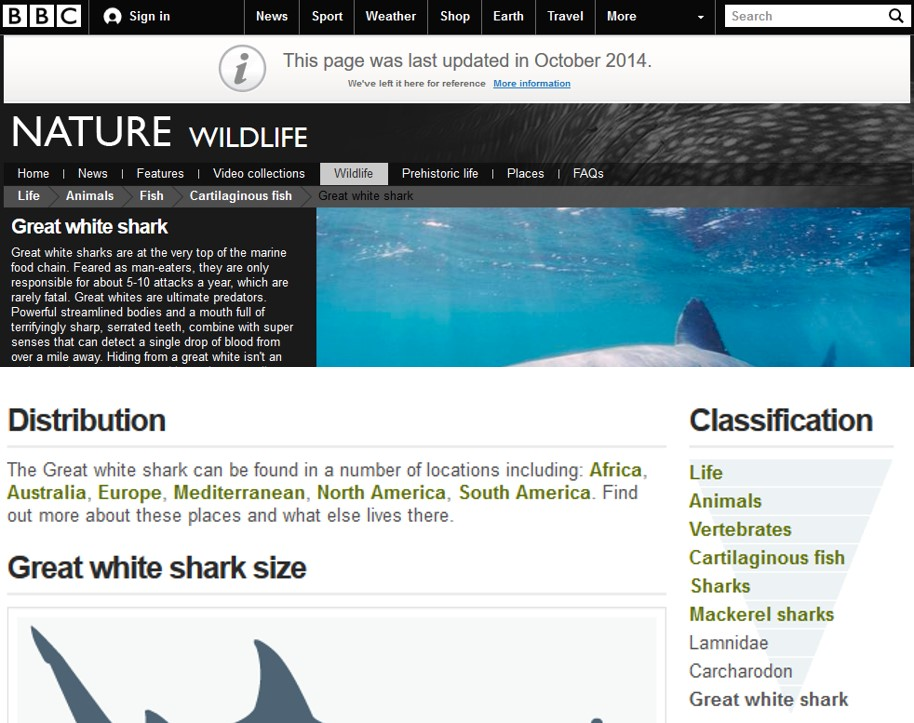
\includegraphics[width=5.0in]{media/ch5/figure-05-03.jpg}
    \caption{Great white shark at BBC: extract of the HTML rendering for
humans}
    \label{fig:ch5.3}
\end{figure}


When accessed by a Web browser for a human the response contains an HTML
page to be displayed (Figure~\ref{fig:ch5.3}) but when accessed by a machine the
response was a redirection to the RDF version of that description
(Figure~\ref{fig:ch5.4}) that could be found here:


\begin{lstlisting}
http://www.bbc.co.uk/nature/life/Great_white_shark.rdf
\end{lstlisting}

\begin{figure}
\begin{lstlisting}
<?xml version="1.0" encoding="utf-8"?><rdf:RDF
    xmlns:rdfs="http://www.w3.org/2000/01/rdf-schema#" 
    xmlns:rdf="http://www.w3.org/1999/02/22-rdf-syntax-ns#" 
    xmlns:owl="http://www.w3.org/2002/07/owl#" 
    xmlns:foaf="http://xmlns.com/foaf/0.1/" 
    xmlns:dc="http://purl.org/dc/terms/" 
    xmlns:dctypes="http://purl.org/dc/dcmitype/" 
    xmlns:skos="http://www.w3.org/2004/02/skos/core#"
    xmlns:xsd="http://www.w3.org/2001/XMLSchema#" 
    xmlns:po="http://purl.org/ontology/po/" 
    xmlns:wo="http://purl.org/ontology/wo/">
    		<rdf:Description rdf:about="/nature/species/Great_white_shark">
		<foaf:primaryTopic rdf:resource="/nature/species/Great_white_shark#species"/>
		<rdfs:seeAlso rdf:resource="/nature/species"/>
	</rdf:Description>
		<wo:Species rdf:about="/nature/life/Great_white_shark#species">
				<rdfs:label>Great white shark</rdfs:label>
				<wo:name rdf:resource="http://www.bbc.co.uk/nature/species/Great_white_shark#name"/>
	<foaf:depiction rdf:resource="http://ichef.bbci.co.uk/naturelibrary/images/ic/640x360/g/gr/great_white_shark/great_white_shark_1.jpg"/>
	<dc:description>Great white sharks are at the very top of the marine food chain. Feared as man-eaters, they are only responsible for about 5-10 attacks
\end{lstlisting}
    \caption{Great white shark at BBC: extract of the RDF/XML version for
machines}
    \label{fig:ch5.4}
\end{figure}

Moving to a completely different domain and data source, let us now
consider UniProt that provides RDF descriptions of protein sequence and
function. Again, if you are a biologist interested in the ``Cell surface
glycoprotein MUC18'', there is a URI for that:

\begin{lstlisting}
http://purl.uniprot.org/uniprot/P43121
\end{lstlisting}


\begin{figure}
    \centering
    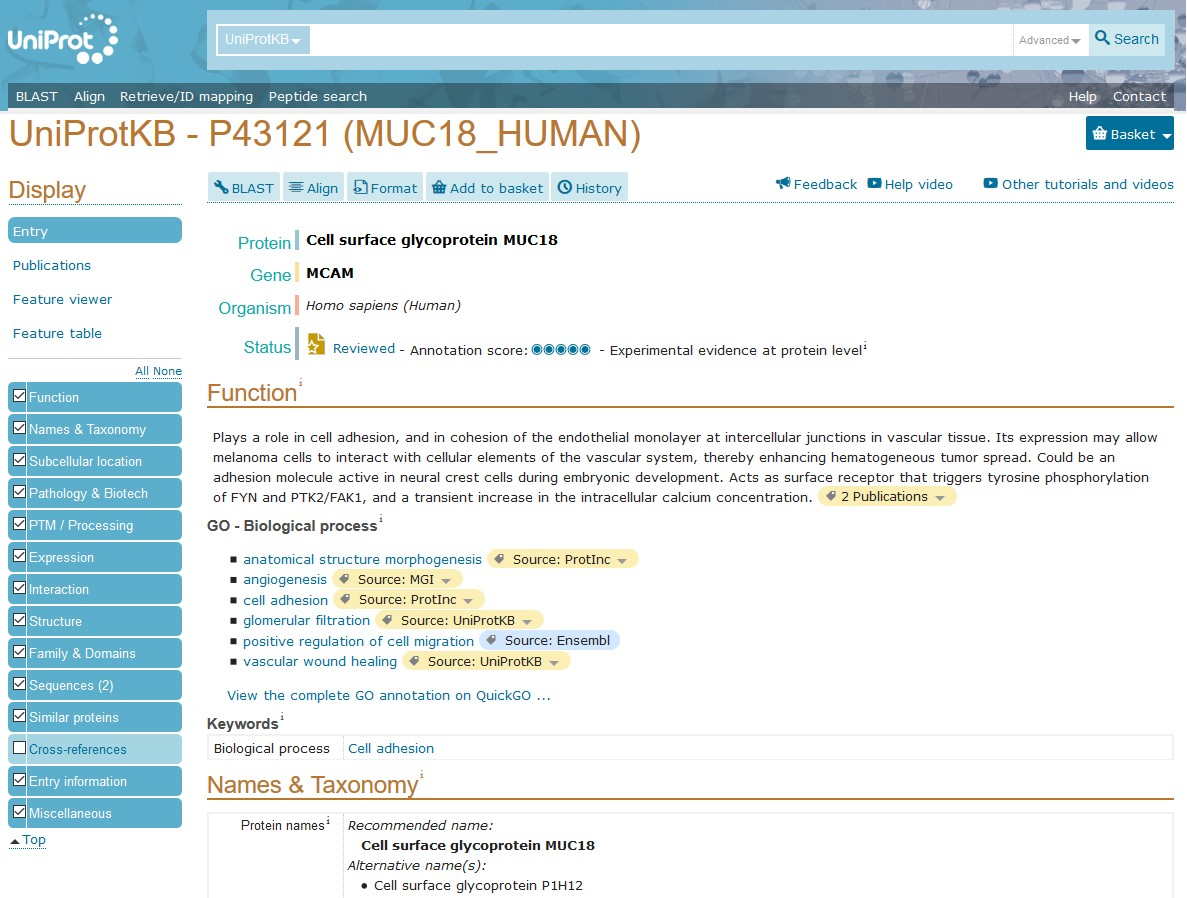
\includegraphics[width=5.0in]{media/ch5/figure-05-05.jpg}
    \caption{Cell surface glycoprotein MUC18 in UnitProt: extract of the HTML
rendering for humans}
    \label{fig:ch5.5}
\end{figure}

When accessed by a Web browser for a human the response contains an HTML
page to be displayed (Figure~\ref{fig:ch5.5}) but when accessed by a machine the
response is a redirection to the RDF version of that description (Figure~\ref{fig:ch5.6} that can be found here:

\begin{lstlisting}
https://www.uniprot.org/uniprot/P43121.rdf
\end{lstlisting}



\begin{figure}
\begin{lstlisting}
<rdf:RDF  (…)>
  <rdf:Description rdf:about="http://purl.uniprot.org/uniprot/P43121">
    <rdf:type rdf:resource="http://purl.uniprot.org/core/Protein"/>
    <reviewed rdf:datatype="http://www.w3.org/2001/XMLSchema#boolean">true</reviewed>
    <created rdf:datatype="http://www.w3.org/2001/XMLSchema#date">1995-11-01</created>
    <modified rdf:datatype="http://www.w3.org/2001/XMLSchema#date">2018-06-20</modified>
    <version rdf:datatype="http://www.w3.org/2001/XMLSchema#int">165</version>
    <mnemonic>MUC18_HUMAN</mnemonic>
    <oldMnemonic>MU18_HUMAN</oldMnemonic>
    <replaces rdf:resource="http://purl.uniprot.org/uniprot/O95812"/>
    <replaces rdf:resource="http://purl.uniprot.org/uniprot/Q59E86"/>
    <replaces rdf:resource="http://purl.uniprot.org/uniprot/Q6PHR3"/>
    <replaces rdf:resource="http://purl.uniprot.org/uniprot/Q6ZTR2"/>
    <citation rdf:resource="http://purl.uniprot.org/citations/2602381" rdf:ID="_P43121-citation-2602381"/>
    <citation rdf:resource="http://purl.uniprot.org/citations/8378324" rdf:ID="_P43121-citation-8378324"/>
    <citation rdf:resource="http://purl.uniprot.org/citations/11709656" rdf:ID="_P43121-citation-11709656"/>
\end{lstlisting}
    \caption{Cell surface glycoprotein MUC18 in UnitProt: extract of the
RDF/XML version for machines}
    \label{fig:ch5.6}
\end{figure}

As a third example let us consider DBpedia, which is according to their
own site, ``a crowd-sourced community effort to extract structured
content from the information created in various Wikimedia projects''
including the famous Wikipedia encyclopaedia. This initiatives extracts
and publicly makes available structured data from the pages of Wikipedia
and other Wikimedia projects, therefore covering a wide variety of
domains and topics. Again they use RDF and linked data principles
therefore every topic has a URI for which you can negotiate HRTML of
RDF. Consider for instance the topic ``Eiffel Tower'' identified by the
following identifier:

\begin{lstlisting}
{http://dbpedia.org/\textbf{resource}/Eiffel\_Tower
\end{lstlisting}

If you access that HTTP URI with a browser, you are redirected to the
following URL

\begin{lstlisting}
http://dbpedia.org/\textbf{page}/Eiffel\_Tower
\end{lstlisting}

This URL displays an HTML page rendering all the data extracted about
that topic and available publicly on the Web as linked data (Figure 7).

\begin{figure}
    \centering
    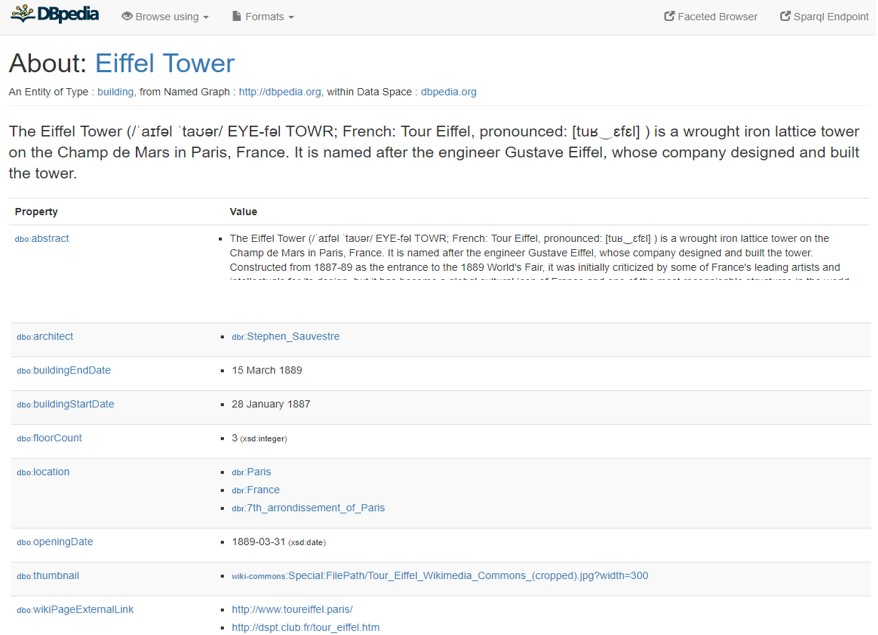
\includegraphics[width=5in]{media/ch5/figure-05-07.jpg}

    \caption{Eiffel Tower at DBpedia: extract of the HTML rendering for humans}
    \label{fig:ch5.7}
\end{figure}

At the same HTTP URI you can negotiate many other formats including, for
instance RDF using Turtle /N3 syntax. You would then be redirected
(Figure 8) to another URL for instance:

\url{http://dbpedia.org/data/Eiffel_Tower.n3}


\begin{figure}
 \begin{lstlisting}
1.	@prefix dbo:	<http://dbpedia.org/ontology/> .
2.	@prefix dbr:	<http://dbpedia.org/resource/> .
3.	@prefix rdf:	<http://www.w3.org/1999/02/22-rdf-syntax-ns#> .
4.	@prefix umbel-rc:	<http://umbel.org/umbel/rc/> .
5.	@prefix dbp:	<http://dbpedia.org/property/>
6.	@prefix wikidata:	<http://www.wikidata.org/entity/> .
7.	dbr:Eiffel_Tower
8.	rdf:type	umbel-rc:Skyscraper, wikidata:Q41176, umbel-rc:Building,
                    dbo:Location, dbo:Place, dbo:Building ;
9.	dbo:buildingStartDate	"28 January 1887" ;
10.	dbp:years	1889 ;
11.	dbo:floorCount	"3"^^xsd:positiveInteger ;
12.	dbp:mainContractor	dbr:Gustave_Eiffel ;
13.	dbo:location	dbr:Paris ,
14.	<http://dbpedia.org/resource/7th_arrondissement_of_Paris> ,
15.	dbr:France ;
16.	dbp:latd	48 ;
17.	dbp:latm	51 ;
18.	dbp:longd	2 ;
19.	dbp:longew	"E"^^rdf:langString ;
20.	dbp:longm	17 ;
21.	dbp:elevatorCount	8 ;
22.	dbp:height	300 .
 \end{lstlisting}
    \caption{Eiffel Tower at DBpedia: extract of the RDF/Turtle version for
machines}
    \label{fig:ch5.8}
\end{figure}

Now let us fully play the game of linked data. In (Figure 8) you can
find a piece of code (line 8) saying that the Eiffel Tower is of type
wikidata:Q41176 which is a qualified name using the prefix ``wikidata''
attached to a namespace (line 6). At this stage we don't know what this
means but we can follow our nose and expand the qualify name by
replacing the prefix with the namespace to obtain an HTTP URI that we
can access

\begin{lstlisting}
http://www.wikidata.org/\textbf{entity}/Q41176
\end{lstlisting}

If you access that HTTP URI with a browser, you are redirected to the
following URL

\begin{lstlisting}
https://www.wikidata.org/\textbf{wiki}/Q41176
\end{lstlisting}


This URL displays an HTML page rendering all the data about that
resource in another important data source of the Web of data: Wikidata
(Figure 9). This is another initiative of Wikimedia that provides as
central storage for the structured data used in other projects of the
foundation projects including Wikipedia, Wikivoyage, etc. This knowledge
base is open on the Web and can be read and edited by both humans and
machines.

\begin{figure}
    \centering
    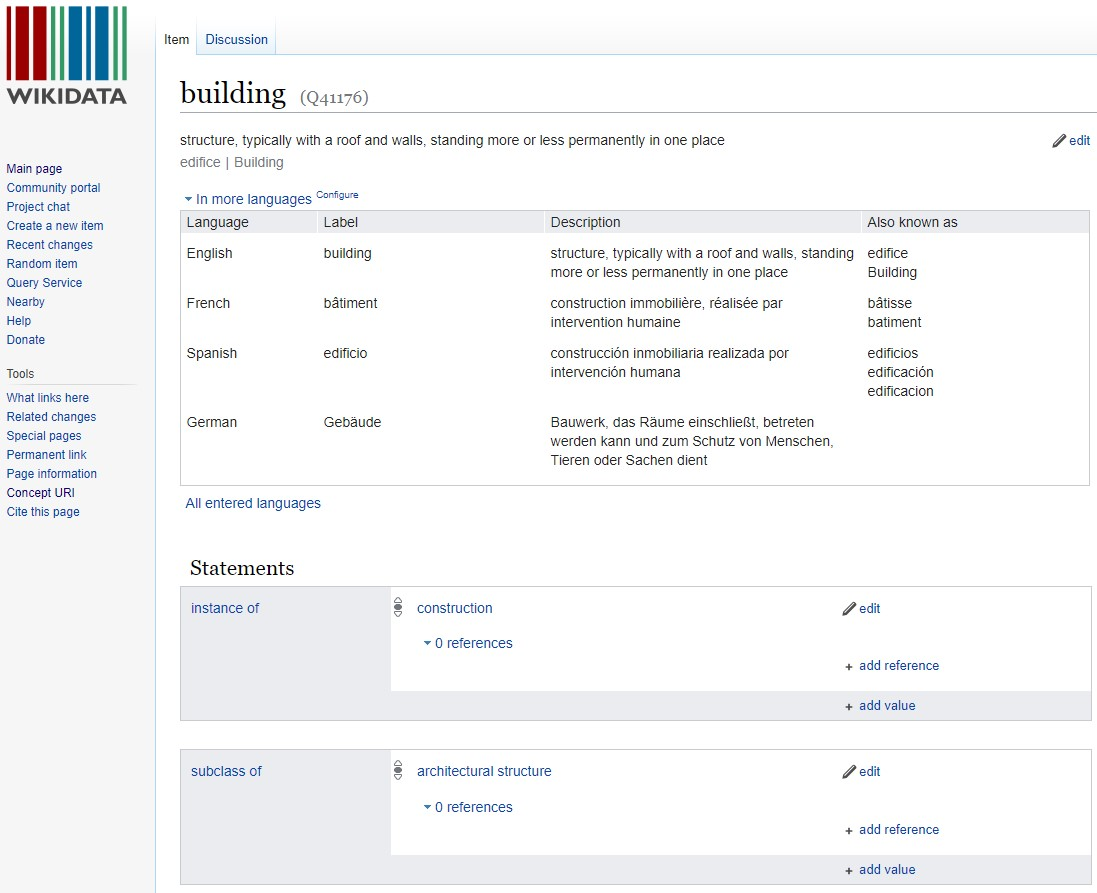
\includegraphics[width=5.0in]{media/ch5/figure-05-09.jpg}
    \caption{``Building'' at Wikidata: extract of the HTML rendering for humans}
    \label{fig:ch5.9}
\end{figure}

Again you can force the access to another format for the same data for
instance in RDF N-Triple (Figure 10). But if we now put all the pieces
together we can see that this mysterious resource called wikidata:Q41176
and found among the types of the Eiffel Tower in DBpedia represents the
category of the buildings in the data of Wikidata. So we see that these
linked data explain that the dataset of DBpedia the Eiffel Tower is
declared to be a Building in the sense of the dataset of Wikidata. We
witness a link across two data sources on the Web of data.

\begin{figure}
 \begin{lstlisting}
<http://www.wikidata.org/entity/Q41176> <http://www.w3.org/2000/01/rdf-schema#label> "building"@en .
<http://www.wikidata.org/entity/Q41176> <http://www.w3.org/2004/02/skos/core#prefLabel> "building"@en .
<http://www.wikidata.org/entity/Q41176> <http://schema.org/name> "building"@en .
<http://www.wikidata.org/entity/Q41176> <http://www.w3.org/2000/01/rdf-schema#label> "Bilding"@pih .
<http://www.wikidata.org/entity/Q41176> <http://www.w3.org/2004/02/skos/core#prefLabel> "Bilding"@pih .
<http://www.wikidata.org/entity/Q41176> <http://schema.org/name> "Bilding"@pih .
<http://www.wikidata.org/entity/Q41176> <http://www.w3.org/2000/01/rdf-schema#label> "budova"@sk .
<http://www.wikidata.org/entity/Q41176> <http://www.w3.org/2004/02/skos/core#prefLabel> "budova"@sk .
\end{lstlisting}
    \caption{Building at Wikidata: extract of the RDF N-Triple version for
machines}
    \label{fig:ch5.10}
\end{figure}

Until now we have used different tricks (different URLs) to see the
different formats available for each description avoiding to perform the
content negotiation ourselves. Let us now mention one way to perform
manually the dereferenciation of an HTTP URI and the content
negotiation. For this, you may use different tools or command and even
do it from a programming language if you want. Here we use the CURL
command line tool and library to transfer data using HTTP URIs. The
command may already be available on your machine or you may have to
install it from the Web site of the software\footnote{\url{https://curl.haxx.se/}}.
As show in Figure 11, this tool allow us to perform calls as command
lines and we performed two executions of CURL here on the same URL from
Wikidata we just saw. The first execution uses CURL with the options
``-o'' to save the output in a file named ``PageBuildings.html''. It
also uses the option ``-L'' to follow redirections and ``-H'' to specify
in the HTTP headers of our call that we want a response in HTML. The
last parameter is the URI of the category Buildings in Wikidata as seen
before. The result shows that CURL makes a first call, as a result it is
redirected to another address and makes a second call from which it
obtains and saves an HTML file of 230 kilobytes. The second execution is
almost the same except we specify in the HTTP headers of our call that
we want a response in RDF/XML and we save this second result in another
file named ``DataBuildings.rdf''. The result shows that again CURL makes
a first call, as a result it is redirected to another address and makes
a second call from which it obtains an RDF/XML file of 1620 kilo bytes

\begin{figure}
    \centering
    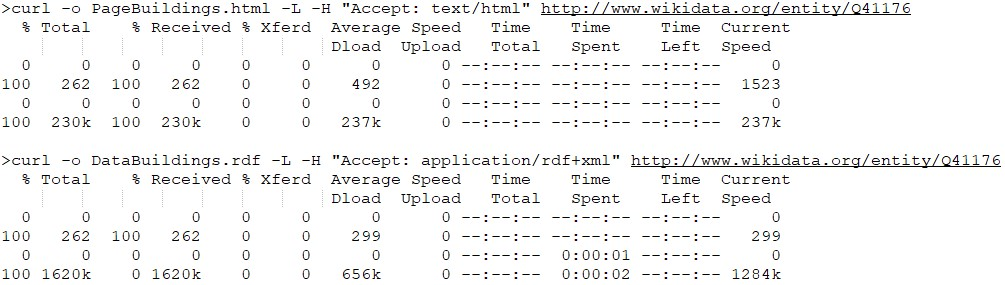
\includegraphics[width=5.0in]{media/ch5/figure-05-11.jpg}
    \caption{Performing CURL calls on Wikidata HTTP URIs to demonstrate
dereferencing and content negotiation}
    \label{fig:ch5.11}
\end{figure}

\hypertarget{linking-rdf-data}{%
\subsection{Linking RDF data}\label{linking-rdf-data}}

The recommended format to publish linked data on the Web is RDF and we
now know it has different serialization formats (XML, Turtle/N3,
JSON-LD, RDFa, etc.) that can be part of the content negotiation when
dereferencing an HTTP URI. The very fact RDF relies on URIs to identify
everything makes it an excellent data model to allow anyone to publish,
exchange and extend descriptions on the Web. The use of HTTP URIs
provide a standard way to obtain and augment data about any encountered
identifier. In fact, an RDF triple contains up to three HTTP URIs
(subject, predicate and object) and each can be used to ``follow our
noses'' and discover new data. Any HTTP URI used in an RDF description
can be looked-up for more information.

While it is true that any piece of RDF already contains links - since
RDF triples are links between a resource and (another) resource or a
literal -- this must be turned into a more specific best practice: to
weave a Web of linked data we need links across datasets which means the
subjects or objects of the triples of the dataset should reuse or link
URIs from other datasets as much as possible in order to generate that
global giant graph of data we want.

If each source was only using its own URIs within its own domain, then
each source would be an isolated island by default and there would be no
Web of data. As soon as external links are established either when the
data are created (e.g. reusing URIs) or after they were generated (e.g.
alignment) this supports the discovery, crawling, integration, browsing,
aggregation, etc. of multiple data sources in a Web of data.

The external links can be established in many different ways. First the
subject or object of the descriptions can reuse URIs from other
datasources. If the things described are already described somewhere
else in a different way, a new source may decide to reuse the URIs to
extend these descriptions; however the dereferenciation here would be
handled by the other site and this would lead to centralization of URIs.

More classically if the descriptions of a source (e.g. a catalog of
products) provide relations (e.g. ``Made In'') to other things (e.g.
geographical places) they may reuse URIs for descriptions about these
others things from other sources (e.g. a geographical linked dataset).
Related to the idea of alignment, the dataset can also provide
equivalence or identity links between URIs to assert for instance that
two different URIs are in fact identifying the same thing and provide
two different addresses to lookup for information about that same thing.

Finally every class or property used in an RDF description is also an
HTTP URI that, when looked up, can provide additional semantics and
support additional inferences. In addition, by reusing existing schemata
a description can be integrated to other datasets using the same
schemata and can be consumed by software that use same schemata. The
reuse of schemata fosters interoperability.

To find the schema of your dreams, like for anything on the Web, there
are Web applications providing directories and search engine
functionality. One of them is called LOV for Linked Open
Vocabularies\footnote{\url{http://lov.okfn.org/}} where you can find the
most well-known vocabularies and their links (Figure)

\begin{figure}
    \centering
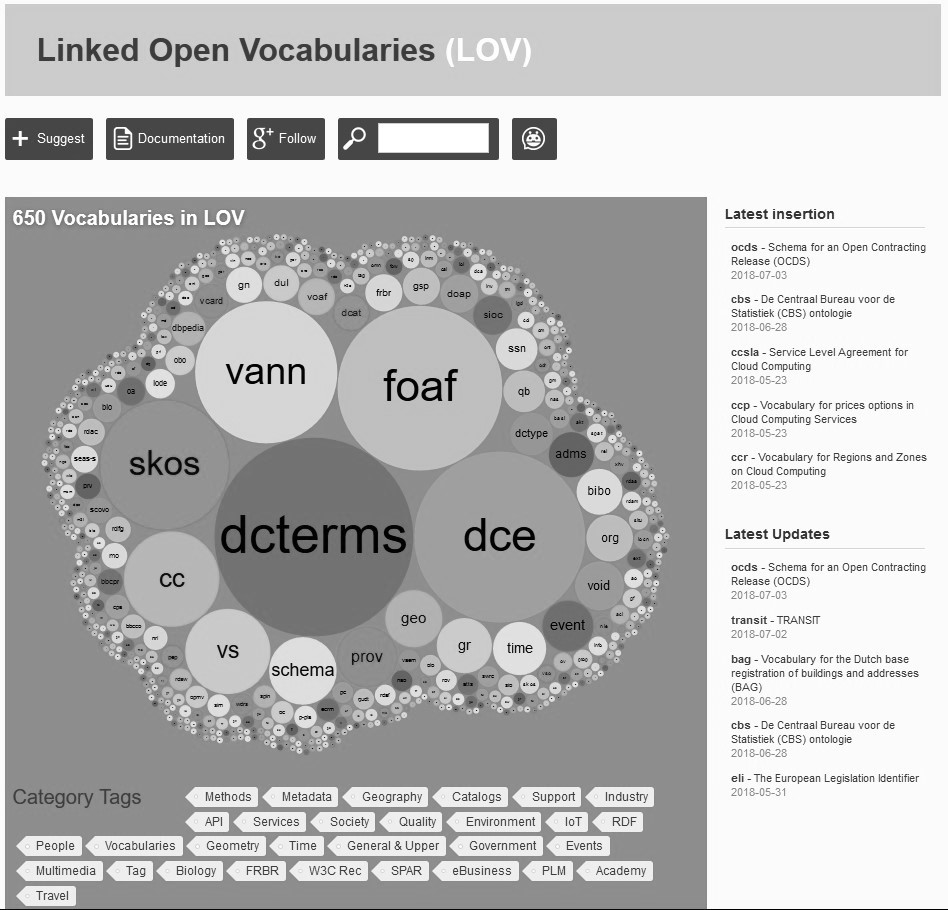
\includegraphics[width=5.0in]{media/ch5/figure-05-12.jpg}
    \caption{Linked Open Vocabularies (LOV) at OKFN}
    \label{fig:ch5.12}
\end{figure}

\hypertarget{cooking-a-web-of-linked-data-the-datatouille-metaphor}{%
\subsection{\texorpdfstring{Cooking a Web of linked data: the
\emph{Datatouille}
metaphor}{Cooking a Web of linked data: the Datatouille metaphor}}\label{cooking-a-web-of-linked-data-the-datatouille-metaphor}}

The overall process for producing and consuming linked data on the Web
may also be explained using a secret of ratatouille recipe. To obtain a
perfect ratatouille dish as cooked in the south of France one of the
tricks is to cook each vegetable separately (stage 1). Once each one is
properly cooked, the chef mixes them and cooks the ratatouille as one
dish (stage 2). Ratatouille is such a versatile dish, that it can be
used as an ingredient for other dishes such as (stage 3).

Preparing, publishing and (re)using linked data has a lot in common with
this process. Each data source is massaged and prepared separately by
its owner and with adequate applications. Each data provider has his own
constraints in terms of data selection (sensitivity, anonymity, etc.),
dataset features (velocity, volume, etc.) and data infrastructure
(legacy software, maintenance cost, etc.). Each source will therefore
cook its linked data separately (stage 1). Then anyone can use and link
to these published data and process them to produce new data: aggregated
data, statistics/mining/inference results, etc. (stage 2). In turn,
these new data become sources that their owners may publish as linked
data on the Web (stage 3).

\begin{figure}

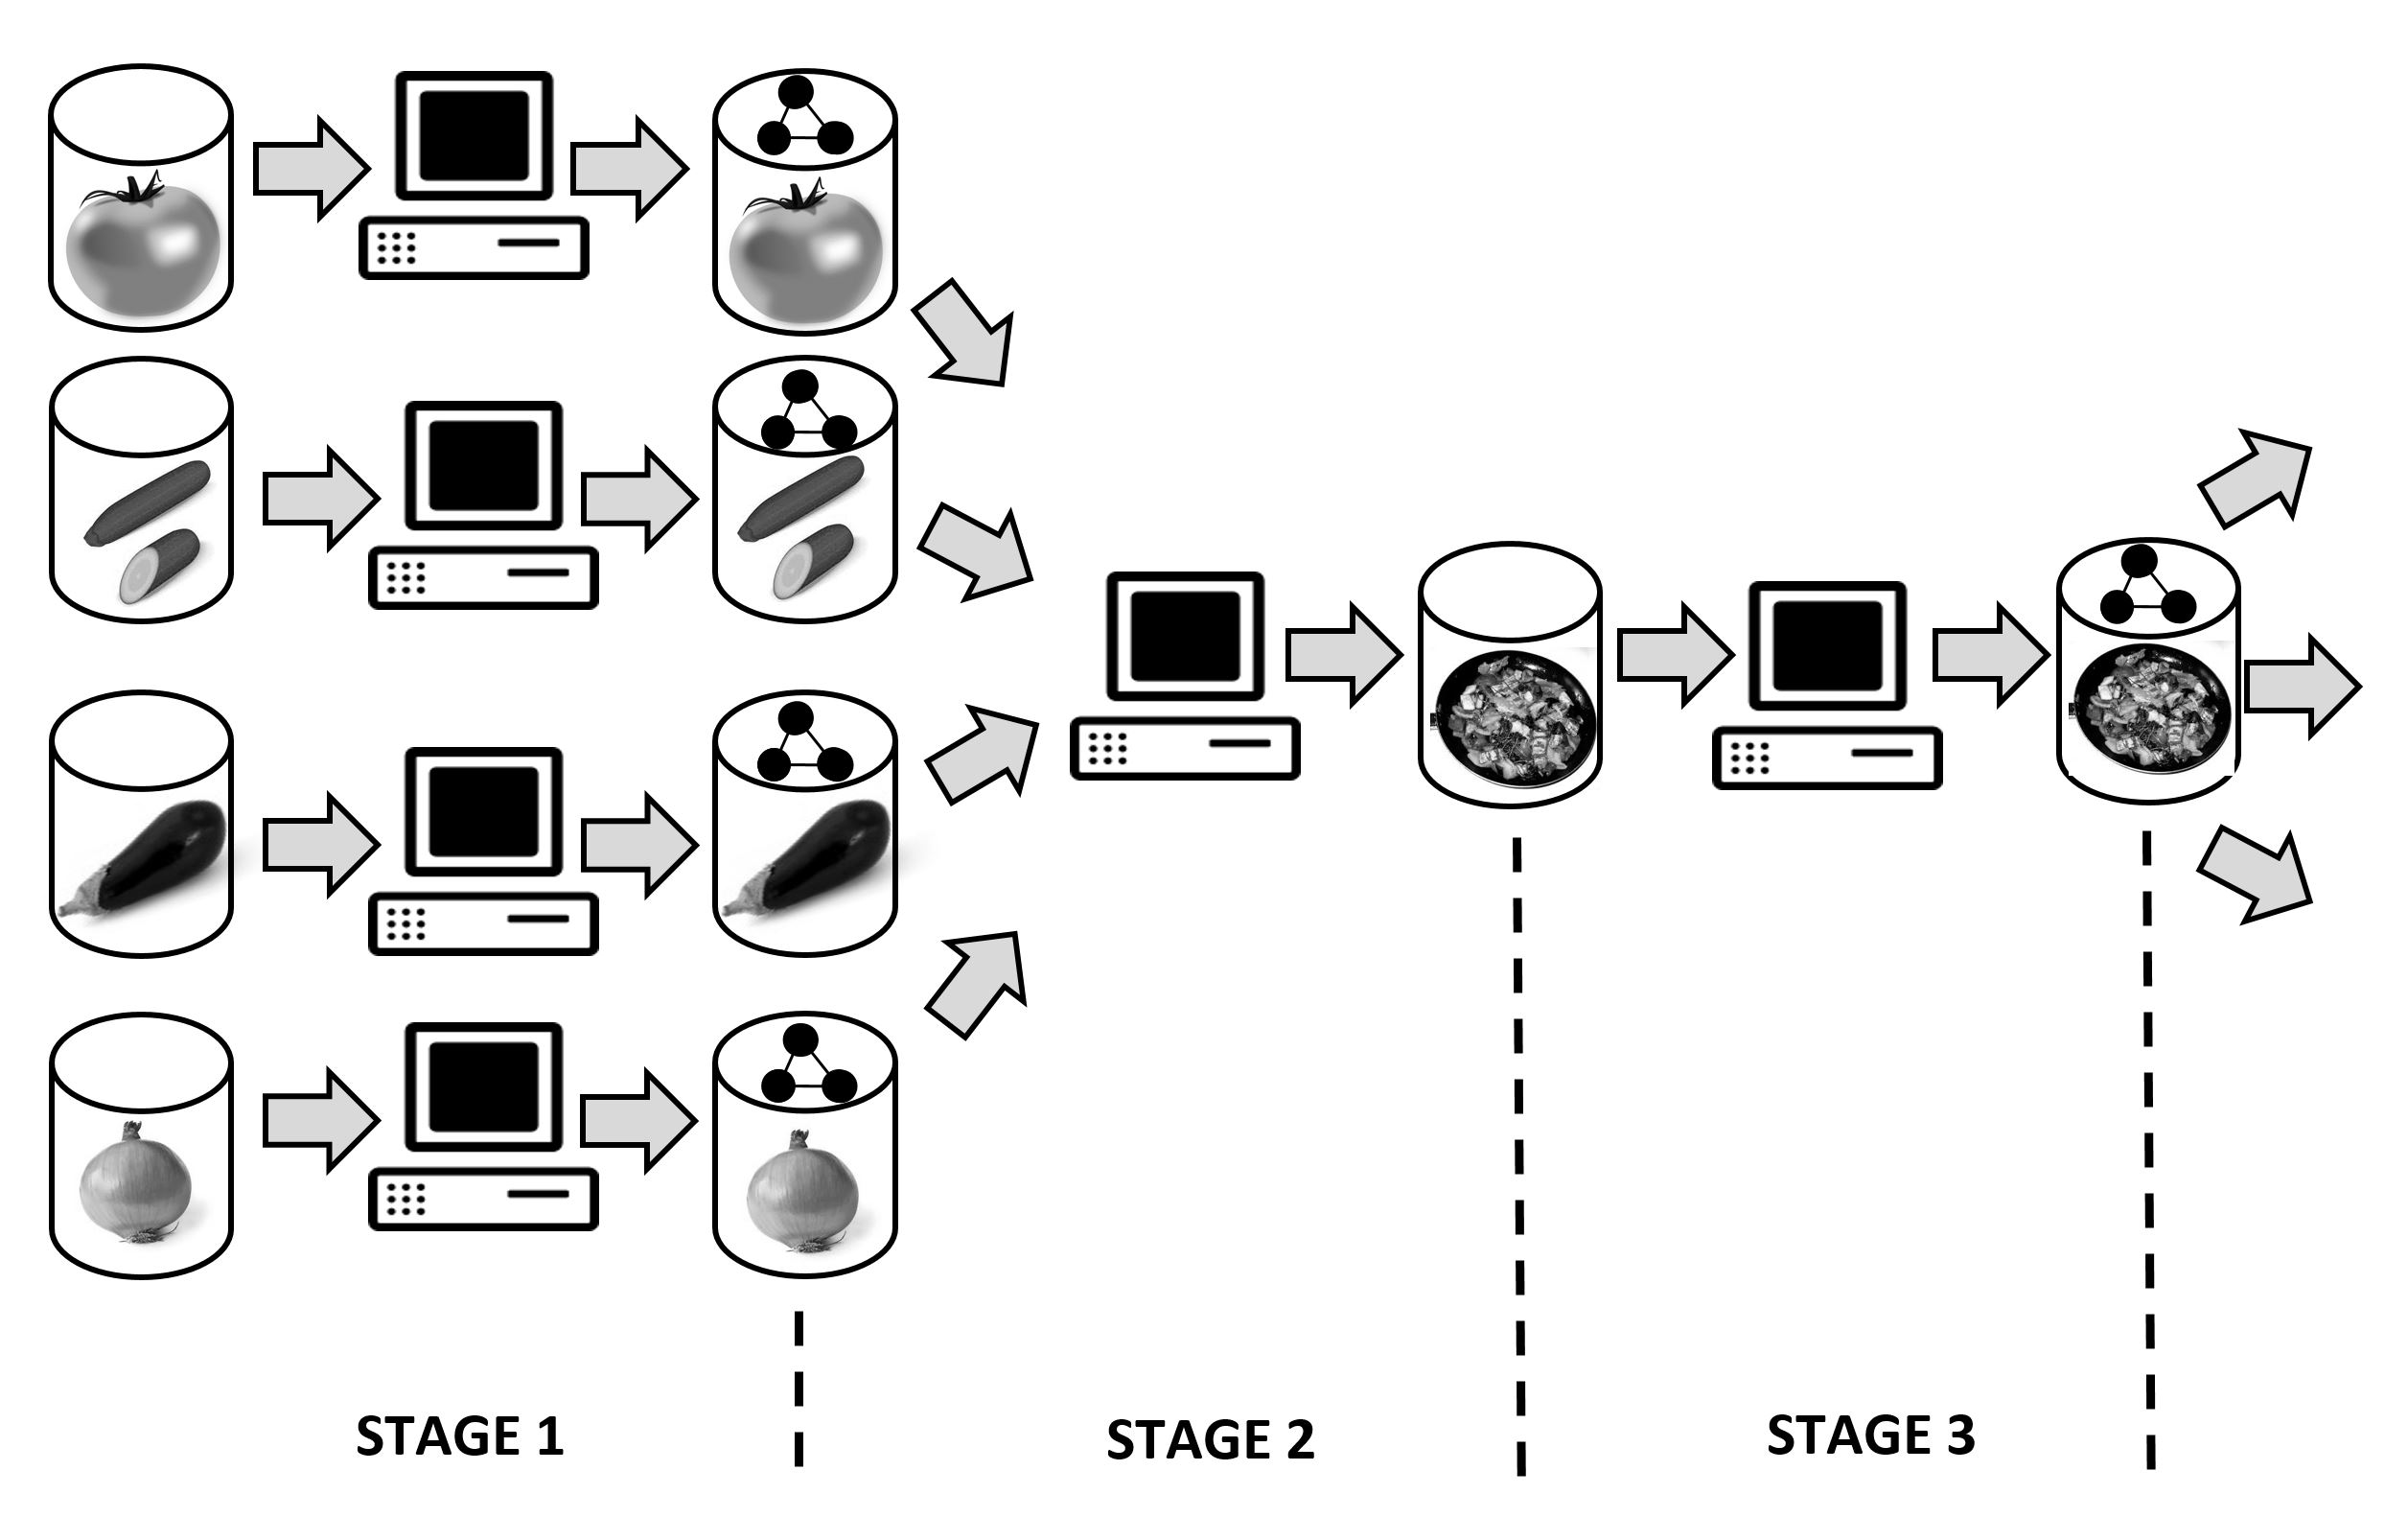
\includegraphics[width=5in]{media/ch5/figure-05-13x}
\label{fig:ch5.13x}
\caption{Three stages in producing linked data.}
\end{figure}

\hypertarget{linked-data-principles-in-a-mug}{%
\subsection{Linked data principles in a
mug}\label{linked-data-principles-in-a-mug}}

The W3C also found a way to summarize the linked data principles and had
it printed on mugs as what is called the 5-star deployment scheme for
Linked Data proposed by Tim Berners-Lee. The scheme is a cumulative list
of rules to lift Web data from one star to five stars. Each additional
rule to gain a star presumes the data meets the all of the previous
rules. The rules are given below and they cumulate to recommend that
data be available on the Web, in a non-proprietary structured format
using open W3C standards and linked to other data:

\begin{figure}
\begin{quote}
$\star{}$ Data is available on the Web, in whatever format.

$\star{}\star{}$ Available as machine-readable structured data, (i.e., not a scanned
image).

$\star\star\star$ Available in a non-proprietary format, (i.e, CSV, not Microsoft
Excel).

$\star\star\star\star$ Published using open standards from the W3C (RDF and SPARQL).

$\star\star\star\star\star$ All of the above and links to other Linked Open Data.
\end{quote}
\caption{Linked data principles from W3C}
\label{fig:ch5.13}
\end{figure}


\hypertarget{yet-another-cloud-for-the-web}{%
\subsection{Yet Another Cloud For the
Web}\label{yet-another-cloud-for-the-web}}

The term ``linked open data cloud'' or ``LOD Cloud'' does not refer to
the cloud paradigm of computer science but to of linked datasets
obtained by applying the linked data principles. This cloud is a graph
formed by nodes representing open datasets and edges indicating that the
data of two datasets are linked i.e. if one of the dataset reuses the
identifiers of the other dataset to identify the same resources (e.g.
persons, places, etc.). This cloud comprises only a small part the Web
of Data, made up of datasets that have declared at the Linked Open Data
Hub Web site, which collects and curates their descriptions before
compiling them into the Linking Open Data cloud diagram as shown in
figure 14.

\begin{figure}
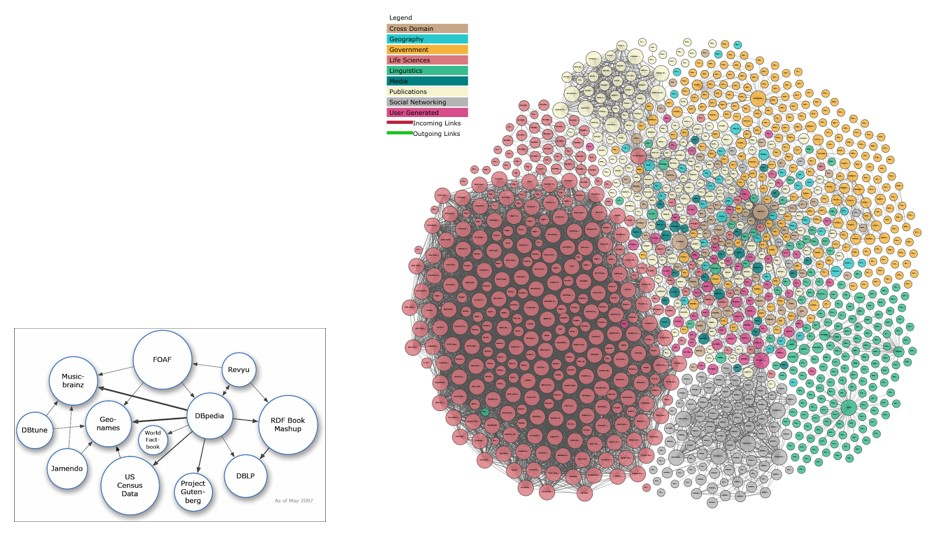
\includegraphics[width=5.0in]{media/ch5/figure-05-14.jpg}
\label{fig:ch5.14}
\caption{Linking Open Data cloud diagrams\protect\footnotemark\ ten years apart from 2007 (left) and 2017 (right)}
\end{figure}
\footnotetext{Andrejs Abele, John
  P. McCrae, Paul Buitelaar, Anja Jentzsch and Richard Cyganiak.
  http://lod-cloud.net/}

The 2017 edition of the diagram shown above shows a LOD cloud
aggregating 150 billion triples from nearly 3000 datasets. Every node
(circle) corresponds to a dataset, some of them very large in their own
right. The different colors show different domains of application (e.g.
life sciences, publication, governmental, geography).

Some of the sources included in this cloud are well-known for being
central, historic or atypical. Let us mention some of them:

\begin{itemize}
\item
  DBPedia is a central and historical source of data and identifiers in
  the linked open data cloud. It is one of the pioneering sources and
  its encyclopedic nature makes it well-suited as a source of reference
  for other datasets. Its name comes from the fact it publishes linked
  structured data extracted from Wikipedia and, in particular, from its
  \emph{infoboxes} (structured tables summarizing facts about a topic in
  a Wikipedia page). DBPedia includes all kinds of data, including birth
  dates of famous people, names of capital cities in different
  languages, geographical coordinates of landmarks, names and
  identifiers of drugs, etc. All of these data are available as linked
  open data.
\item
  Wikidata is an initiative of the Wikimedia foundation to crowdsource
  the contribution and maintenance of a central storage for the
  structured data to be used in other foundation projects including
  Wikipedia, Wikivoyage, etc. Here the approach is not to extract data
  from other sources but to directly edit and curate structured data in
  a Wiki manner. Then this structured data sources can be queried to
  generate content such a as tables or infoboxes in other sites. Again,
  all of these data are available as linked open data.
\item
  Geonames is a free geographical database that covers all countries
  and, at the time of this writing, contains over eleven million place
  descriptions (countries, cities, regions, etc.) with their names and
  information including currency, population, language, area,
  geographical coordinates, etc.
\item
  UniProt stands for Universal Protein Resource and is an international
  initiative to build and publish a comprehensive dataset of protein
  sequences and annotations.
\end{itemize}

In this book we included a number of examples from the Web such as the
data sources we just mentioned. At the time of writing these sources ae
available but anything can change on the Web at any moment and we
included several of them not only to show the variety but also to
account for the fact that some of them may change, move or even
disappear by the time you read these lines.

\hypertarget{validating-data}{%
\subsection{Validating data}\label{validating-data}}

Applications that publish and consume data from the Web of data are
written and hosted by very different organizations. Validation is a way
to ensure interoperability between open and heterogeneous as the ones
the Web architecture now links. Moreover, one of the strengths of RDF is
the simplicity and genericity of its standard graph data model but, as a
result, it is used to represent a huge variety of data and that variety
is one of the issues when processing big data. This means that the
quality of the data you will get may vary a lot from one source to
another. When discovering and exchanging data over the Web we therefore
need to check whether the data we obtain match what we expect in terms
of content and structure. This is also true when obtaining data from
users. In designing interactions with a user it is important to know
what information is mandatory and the constraints that must be met for
the input to be valid. If the user is entering their personal data, you
may want to check that the family name and first name have been provided
properly. If they are taking orders, you may want to ensure the product
ID and the quantity have been appropriately filled in, etc. All these
are examples of use cases for an RDF validation mechanism that allows us
to validate the data before adding them to our databases.

SHACL (Shapes Constraint Language) addresses the issue of data quality
at the structural level by providing a language to describe the
``shapes'' of the data you are expecting. This takes the form of an RDF
description of the constraints you want to enforce on the data,
including the required properties and the types of values you expect.
Once you have defined your constraints on the RDF data you are
interested in, you can check any piece of data from any source using a
validation software.

Imagine you design an application for collecting user profiles from the
Web. \emph{FOAF} (which stands for \emph{Friend of a Friend}) is a
popular vocabulary for representing user profile data on the Web of
data. Suppose that every time your application finds such a FOAF profile
on the Web, it wants to check its completeness with respect to some
requirements. As shown in Figure~\ref{fig:ch5.15}, the conditions are themselves
expressed in RDF and the core notion is the ``shape'' providing a
description that the data graphs need to satisfy. In our example, we
declare a shape (line 5) that targets resources of type foaf:Person
(line 7) and specified three constraints we would like to enforce. The
first constraint (lines 8-15) makes it compulsory to have exactly one
family name that must be a string of characters. The second constraint
(lines 16-24) makes it compulsory to have a gender and this must have
for value either ``male'' or ``female''. The third constraint (lines
25-28) just ensures that if the homepage is provided it is a valid IRI.

\begin{figure}
\begin{lstlisting}
1.	@prefix foaf: <http://xmlns.com/foaf/0.1/> .
2.	@prefix sh: <http://www.w3.org/ns/shacl#> .
3.	@prefix xsd: <http://www.w3.org/2001/XMLSchema#> .
4.	
5.	:PersonShape
6.	    a sh:NodeShape ;
7.	    sh:targetClass foaf:Person ;
8.	    sh:property [
9.	        sh:path foaf:familyName ;
10.	        sh:name "family name" ;
11.	        sh:description "the family name of a 
                                          person." ;
12.	        sh:datatype xsd:string ;
13.	        sh:maxCount 1 ;
14.	        sh:minCount 1 ;
15.	    ] ;
16.	    sh:property [
17.	        sh:path foaf:gender ;
18.	        sh:name "gender" ;
19.	        sh:description "the gender of a person 
                                 ('male' or 'female')." ;
20.	        sh:datatype xsd:string ;
21.	        sh:maxCount 1 ;
22.	        sh:minCount 1 ;
23.		sh:pattern "^(male|female)$" ;
24.	    ] ;
25.		sh:property [                
26.			sh:path foaf:homepage ;
27.			sh:nodeKind sh:IRI ;
28.		] .
\end{lstlisting}
\label{fig:5.15}
\caption{A SHACL shape to validate FOAF data: the shape is represented
itself in RDF.}
\end{figure}


If you provide such a SHACL shape to a SHACL validator, you can then
check if some data is valid with respect to these constraints. Consider
the data in Figure 16 containing two small FOAF profiles for Bob (lines
3-5) and Alice (lines 7-11). If you run a validator on these data the
report indicates that Alice is a valid foaf:Person according to your
constraints but that Bob is missing the gender property.

\begin{figure}
\begin{lstlisting}
1.	@prefix foaf: <http://xmlns.com/foaf/0.1/> .
2.	
3.	:Bob a foaf:Person ;
4.	    foaf:firstName "Robert" ;
5.	    foaf:familyName "Doe" .
6.	
7.	:Alice a foaf:Person ;
8.	    foaf:firstName "Alice" ;
9.	    foaf:familyName "Doe" ;
10.	    foaf:gender "female" ;
11.	    foaf:homepage <http://alice.homepage.com/> .
\end{lstlisting}
\label{fig:5.16}
\caption{Two FOAF profiles to be validated with the SHACL shape of Figure~\ref{fig:ch5.15}}
\end{figure}



SHACL provides a standard to specify structural patterns to be checked
upon the data by expressing rules about how actual RDF graphs or
subgraphs should look like in your data. This validation happens at the
structural level of the RDF graphs before considering any kind of
semantics or inference as we will see in the chapters about RDFS and
OWL. These structural constraints are already very useful to validate
and integrate data, to document data models, to generate user interfaces
or even code.

\hypertarget{the-linked-data-platform-architecture}{%
\subsection{The Linked Data Platform
architecture}\label{the-linked-data-platform-architecture}}

\emph{Representational State Transfer} (\emph{REST}) is a popular
software architecture style for creating and publishing services on the
Web. REST defines a set of constraints to ensure service
interoperability over the Web, based on accessing and manipulating
representations of resources through a uniform and predefined set of
operations (in particular, the standard HTTP methods \emph{GET},
\emph{PUT}, \emph{PATCH}, \emph{POST}, and \emph{DELETE}). A service
that complies with the REST principles is said to be \emph{RESTful}.

In a similar way, the W3C has defined the Linked Data Platform (LDP)
that specifies how web applications can publish, edit and delete
resources using the HTTP protocol. It can be seen as a standardized REST
access to linked data, describing how to build clients and servers that
create, read, and write linked data Resources.

Because in real applications you have to manage a variety of files and
data formats, LDP distinguishes two kinds of resources: resources with
an RDF representation (RDF descriptions) and resources using other
formats (e.g. HTML files, images, binary files).

In order to be able to add or remove resources from the Web, you need to
have some kind of data space in which to read and write these resources.
For this reason, LDP also introduces the notion of \emph{containers} to
group and manage resources. A container is collections of resources,
often homogeneous ones (e.g. a collection of user profiles, a catalog of
book descriptions, an inventory of cars). LDP supports three kinds of
containers with more or less support to automate the creation of
membership relations between the resources and their containers. A
\emph{Basic Container} provides a simple containment vocabulary and
access mechanism. A \emph{Direct Container} supports the use of a
domain-specific membership assertions (e.g. assert a relation called
``author'' between all the resources of a collection of books and a
resource representing their author). An \emph{Indirect Container} allows
you to control more precisely the URI of the domain-specific member
resources you create.

LDP specifies the effect that each HTTP verb has on resources and
containers. Figure 17 summarizes each case and shows how these standard
methods allow you to use only HTTP to remotely manage resources and
containers in any LDP-compliant platform.


\begin{figure}
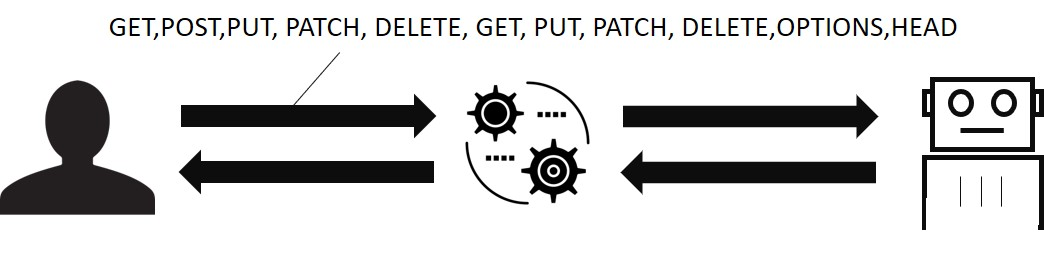
\includegraphics[width=5.0in]{media/ch5/figure-05-17.jpg}
\begin{tabular}{|lll|}
\hline
\textbf{Resource type} & \textbf{Method} & \textbf{Result}\tabularnewline
\hline\hline
Container & GET & Lists all the members of the container\tabularnewline
& POST & Create a new member of the container\tabularnewline
& PUT & Update the description of the container\tabularnewline
& PATCH & Partial update of the description of the
container\tabularnewline
& DELETE & Delete the container\tabularnewline
\hline
Any other resource type & GET & Retrieve a representation of the
resource\tabularnewline
& PUT & Update the resource description\tabularnewline
& PATCH & Partial update of the resource description\tabularnewline
& DELETE & Delete the resource description\tabularnewline
\hline\hline
Container or resource & OPTIONS & Discover the allowed operations over a
resource\tabularnewline
& HEAD & Only retrieve meta-information about a resource\tabularnewline
\hline
\end{tabular}
 \label{fig:ch5.17}
 \caption{The effects of HTTP verbs as specified in LDP}
\end{figure}


Figure~\ref{fig:ch5.18} shows the transcript of an HTTP request (lines 1-13) sent to a
container (/fabien/, line 1) on an LDP platform on a Web server
(inria.fr). The request uses the verb POST (line 1). As we saw in Figure
17, POST to a container creates a new member of that container. The
request provides the description of the RDF resource in Turtle
(serialization specified in line 4) and directly includes the data for
the new resource in the request itself (lines 7-13). The result (lines
15-18) shows that the request was accepted by the server (line 16), the
resource was created (also line 16), and it provides the URI of the
newly created description is returned (line 17).

\begin{figure}
  
    \label{fig:ch5.18}
\begin{lstlisting}
1.	POST /fabien/ HTTP/1.1
2.	Host: inria.fr
3.	Link: <http://www.w3.org/ns/ldp#Resource>; rel="type"
4.	Content-Type: text/turtle
5.	Slug: foaf
6.	
7.	@prefix foaf: <http://xmlns.com/foaf/0.1/> .
8.	@prefix dc: <http://purl.org/dc/terms/> .
9.	<> a foaf:PersonalProfileDocument;
10.	   foaf:primaryTopic <#me> ;
11.	   dc:title 'Fabien’s FOAF profile' .
12.	<#me> a foaf:Person;
13.	   foaf:name 'Fabien Gandon' .
14.	 
15.	 
16.	HTTP/1.1 201 Created
17.	Location: http://inria.fr/fabien/foaf
18.	Link: <http://www.w3.org/ns/ldp#Resource>; rel="type"
19.	Content-Length: 0

\end{lstlisting}
  \caption{Example of a POST request on an LDP container and its result}
  \end{figure}

\hypertarget{summary}{%
\subsection{Summary}\label{summary}}

To weave a Web of linked data you must follow three rules: (1) use HTTP
URIs to name everything (2) provide descriptive information in
appropriate formats about the resources identified by these URIs every
time they are accessed, and (3) include, in these descriptions, links to
HTTP URIs of other things. We have seen how to mint the URIs and how
HTTP can be used to negotiate the best answer when dereferencing a URI.
Web agents may need to validate data that comes from the Web or its
users. For this purpose, the Semantic Web stack provides SHACL, a
language for specifying ``shapes'' for data, which specify structural
constraints to be met by a piece of RDF to be valid. Finally, we saw how
the Linked Data Platform (LDP) provides a standardized service
architecture and set of operations based on HTTP verbs to read and write
resources and resource descriptions on the Web of data.

\hypertarget{fundamental-concepts}{%
\subsection{Fundamental concepts}\label{fundamental-concepts}}

The following fundamental concepts were introduced in this chapter:

\begin{itemize}
\item
  HTTP URIs and dereferencing: a URIs created to name anything but that
  uses the HTTP in order to be dereferenceable by just making and HTTP
  call to the address it provides.
\item
  the content negotiation in HTTP allowing a server to serve for the
  same HTTP URI different contents to Web clients.
\item
  SHACL shapes to validate RDF data at the structural level by providing
  the constraint you expect them to meet.
\item
  Linked Data Platform (LDP) that specifies how web applications can
  publish, edit and delete resources using the HTTP protocol.
\end{itemize}

